\documentclass{article}

  % packages
    % basic stuff for rendering math
    \usepackage[letterpaper, top=1in, bottom=1in, left=1in, right=1in]{geometry}
    \usepackage[utf8]{inputenc}
    \usepackage[english]{babel}
    \usepackage{amsmath} 
    \usepackage{amssymb}
    \usepackage{natbib}

    % extra math symbols and utilities
    \usepackage{mathtools}        % for extra stuff like \coloneqq
    \usepackage{mathrsfs}         % for extra stuff like \mathsrc{}
    \usepackage{centernot}        % for the centernot arrow 
    \usepackage{bm}               % for better boldsymbol/mathbf 
    \usepackage{bbm}              % for indicator functions
    \usepackage{enumitem}         % better control over enumerate, itemize
    \usepackage{hyperref}         % for hypertext linking
    \usepackage{xr-hyper}
    \usepackage{fancyvrb}         % for better verbatim environments
    \usepackage{newverbs}         % for texttt{}
    \usepackage{xcolor}           % for colored text 
    \usepackage{listings}         % to include code
    \usepackage{lstautogobble}    % helper package for code
    \usepackage{parcolumns}       % for side by side columns for two column code
    \usepackage{algorithm}
    \usepackage{algpseudocode}

    % page layout
    \usepackage{fancyhdr}         % for headers and footers 
    \usepackage{uniquecounter} 
    \usepackage{lastpage}         % to include last page number in footer 
    \usepackage{parskip}          % for no indentation and space between paragraphs    
    \usepackage[T1]{fontenc}      % to include \textbackslash
    \usepackage{footnote}
    \usepackage{etoolbox}

    % for custom environments
    \usepackage{tcolorbox}        % for better colored boxes in custom environments
    \tcbuselibrary{breakable}     % to allow tcolorboxes to break across pages

    % figures
    \usepackage{pgfplots}
    \pgfplotsset{compat=1.18}
    \usepackage{float}            % for [H] figure placement
    \usepackage{tikz}
    \usepackage{tikz-cd}
    \usepackage{circuitikz}
    \usetikzlibrary{positioning, shapes, arrows, fit, calc}
    \usepackage{graphicx}
    \usepackage{caption} 
    \usepackage{subcaption}
    \captionsetup{font=small}

    % for tabular stuff 
    \usepackage{dcolumn}

    \usepackage[nottoc]{tocbibind}
    \pdfsuppresswarningpagegroup=1
    \hfuzz=5.002pt                % ignore overfull hbox badness warnings below this limit

  % New and replaced operators
    \DeclareMathOperator{\Tr}{Tr}
    \DeclareMathOperator{\Sym}{Sym}
    \DeclareMathOperator{\Span}{span}
    \DeclareMathOperator{\elbo}{ELBO}
    \DeclareMathOperator{\std}{std}
    \DeclareMathOperator{\Cov}{Cov}
    \DeclareMathOperator{\Var}{Var}
    \DeclareMathOperator{\proj}{proj}
    \DeclareMathOperator{\Corr}{Corr}
    \DeclareMathOperator{\pos}{pos}
    \DeclareMathOperator*{\argmin}{\arg\!\min}
    \DeclareMathOperator*{\argmax}{\arg\!\max}
    \newcommand{\ket}[1]{\ensuremath{\left|#1\right\rangle}}
    \newcommand{\bra}[1]{\ensuremath{\left\langle#1\right|}}
    \newcommand{\braket}[2]{\langle #1 | #2 \rangle}
    \newcommand{\qed}{\hfill$\blacksquare$}     % I like QED squares to be black 

  % Custom Environments
    \newtcolorbox[auto counter, number within=section]{question}[1][]
    {
      colframe = orange!25,
      colback  = orange!10,
      coltitle = orange!20!black,  
      breakable, 
      title = \textbf{Question \thetcbcounter ~(#1)}
    }

    \newtcolorbox[auto counter, number within=section]{exercise}[1][]
    {
      colframe = teal!25,
      colback  = teal!10,
      coltitle = teal!20!black,  
      breakable, 
      title = \textbf{Exercise \thetcbcounter ~(#1)}
    }
    \newtcolorbox[auto counter, number within=section]{solution}[1][]
    {
      colframe = violet!25,
      colback  = violet!10,
      coltitle = violet!20!black,  
      breakable, 
      title = \textbf{Solution \thetcbcounter}
    }
    \newtcolorbox[auto counter, number within=section]{lemma}[1][]
    {
      colframe = red!25,
      colback  = red!10,
      coltitle = red!20!black,  
      breakable, 
      title = \textbf{Lemma \thetcbcounter ~(#1)}
    }
    \newtcolorbox[auto counter, number within=section]{theorem}[1][]
    {
      colframe = red!25,
      colback  = red!10,
      coltitle = red!20!black,  
      breakable, 
      title = \textbf{Theorem \thetcbcounter ~(#1)}
    } 
    \newtcolorbox[auto counter, number within=section]{proposition}[1][]
    {
      colframe = red!25,
      colback  = red!10,
      coltitle = red!20!black,  
      breakable, 
      title = \textbf{Proposition \thetcbcounter ~(#1)}
    } 
    \newtcolorbox[auto counter, number within=section]{corollary}[1][]
    {
      colframe = red!25,
      colback  = red!10,
      coltitle = red!20!black,  
      breakable, 
      title = \textbf{Corollary \thetcbcounter ~(#1)}
    } 
    \newtcolorbox[auto counter, number within=section]{proof}[1][]
    {
      colframe = orange!25,
      colback  = orange!10,
      coltitle = orange!20!black,  
      breakable, 
      title = \textbf{Proof. }
    } 
    \newtcolorbox[auto counter, number within=section]{definition}[1][]
    {
      colframe = yellow!25,
      colback  = yellow!10,
      coltitle = yellow!20!black,  
      breakable, 
      title = \textbf{Definition \thetcbcounter ~(#1)}
    } 
    \newtcolorbox[auto counter, number within=section]{example}[1][]
    {
      colframe = blue!25,
      colback  = blue!10,
      coltitle = blue!20!black,  
      breakable, 
      title = \textbf{Example \thetcbcounter ~(#1)}
    } 
    \newtcolorbox[auto counter, number within=section]{code}[1][]
    {
      colframe = green!25,
      colback  = green!10,
      coltitle = green!20!black,  
      breakable, 
      title = \textbf{Code \thetcbcounter ~(#1)}
    } 
    \newtcolorbox[auto counter, number within=section]{algo}[1][]
    {
      colframe = green!25,
      colback  = green!10,
      coltitle = green!20!black,  
      breakable, 
      title = \textbf{Algorithm \thetcbcounter ~(#1)}
    } 
    
    \definecolor{dkgreen}{rgb}{0,0.6,0}
    \definecolor{gray}{rgb}{0.5,0.5,0.5}
    \definecolor{mauve}{rgb}{0.58,0,0.82}
    \definecolor{darkblue}{rgb}{0,0,139}
    \definecolor{lightgray}{gray}{0.93}
    \renewcommand{\algorithmiccomment}[1]{\hfill$\triangleright$\textcolor{blue}{#1}}

    % default options for listings (for code)
    \lstset{
      autogobble,
      frame=ltbr,
      language=Python,                           % the language of the code
      aboveskip=3mm,
      belowskip=3mm,
      showstringspaces=false,
      columns=fullflexible,
      keepspaces=true,
      basicstyle={\small\ttfamily},
      numbers=left,
      firstnumber=1,                        % start line number at 1
      numberstyle=\tiny\color{gray},
      keywordstyle=\color{blue},
      commentstyle=\color{dkgreen},
      stringstyle=\color{mauve},
      backgroundcolor=\color{lightgray}, 
      breaklines=true,                      % break lines
      breakatwhitespace=true,
      tabsize=3, 
      xleftmargin=2em, 
      framexleftmargin=1.5em, 
      stepnumber=1
    }

  % Page style
    \pagestyle{fancy}
    \fancyhead[L]{Linear Regression}
    \fancyhead[C]{Muchang Bahng}
    \fancyhead[R]{Spring 2024} 
    \fancyfoot[C]{\thepage / \pageref{LastPage}}
    \renewcommand{\footrulewidth}{0.4pt}          % the footer line should be 0.4pt wide
    \renewcommand{\thispagestyle}[1]{}  % needed to include headers in title page

\begin{document}

  \tikzset{
    node_style/.style={
        circle,
        draw=black,
        thick,
        minimum size=20pt,
        inner sep=2pt
    },
    edge_style/.style={
        ->,
        >=latex,
        thick
    },
    runner_node/.style={
        circle,
        draw=black,
        thick,
        minimum size=25pt,
        inner sep=2pt,
        fill=gray!20
    },
    factor_node/.style={
        rectangle,
        draw=black,
        thick,
        minimum size=20pt,
        inner sep=2pt,
        fill=blue!10
    },
    outcome_node/.style={
        circle,
        draw=black,
        thick,
        minimum size=25pt,
        inner sep=2pt,
        fill=green!10
    },
    edge_style/.style={
        ->,
        >=latex,
        thick
    }
  }

\title{Linear Regression}
\author{Muchang Bahng}
\date{Spring 2024}

\maketitle
\tableofcontents
\pagebreak

This covers computability theory, complexity theory, and automata theory. 
Alphabet. Boolean logic


\section{Low-Dimensional Ordinary Least Squares}

  When you learn linear regression for the first time, you are really learning a very specific part of linear regression called ordinary least squares, which is the linear model that comes with a very specific loss function. 

  \begin{definition}[Mean Squared Error Loss]
    The \textbf{MSE loss} is defined 
    \begin{equation}
      L(y, x) = (y - f(x))^2
    \end{equation}
  \end{definition}

  \begin{definition}[Ordinary Least Squares Regression]
    The \textbf{OLS linear regression} model is a linear regression model that tells us to minimize the MSE loss. 
  \end{definition}

  \begin{theorem}[Prediction Risk]
    The \textbf{prediction risk}\footnote{This is a bit different from how Wasserman defines it in his lectures, but I think this is better.} of $f$ is 
    \begin{equation}
      R(f) = \mathbb{E}_{x, y} [ (y - f(x))^2 ] = \int (y - f(x))^2 \,dP(x, y)
    \end{equation}
    and the empricial risk is 
    \begin{equation}
      \hat{R}(f) = \frac{1}{n} \sum_{i=1}^n (y^{(i)} - f(x^{(i)}))^2 
    \end{equation}
  \end{theorem}

  This is a bit weird, since we are just \textit{given} a loss function rather than having derived one from our model. There are two paths that we can take to derive this loss function. 
  \begin{enumerate}
    \item The first is to have the extra convenient assumption that the errors $\epsilon$ are Gaussian. This is not too unrealistic since combinations of many random noise gives us a Gaussian by the CLT. As often done in machine learning, by computing the likelihood, we can take its negative logarithm to get our loss. 
    \item The second does \textit{not} assume a distribution on $\epsilon$ and rather uses the Gauss-Markov theorem to directly say that the MSE loss minimizes variance among unbiased estimators. This is in a sense more fundamental. 
  \end{enumerate}
  Sometimes, the Gaussian error is given as an assumption, and sometimes it is not. We will go through all these points by first talking about the nice bias-variance decomposition of the MSE loss. Then, we will use the Gauss-Markov theorem justify the MSE loss and introduce the least-squares solution. Finally, we will look at the likelihood approach using Gaussian residuals. 

\subsection{Least Squares Solution} 

  Note that we have assumed that $\mathbf{X}^T \mathbf{X}$ was invertible in order for such a solution to be unique, i.e. $\mathbf{X}$ must be full rank. This process breaks down when it isn't invertible, e.g. if there are repetitions in the features (one feature is a linear combination of the others and hence not full column rank). We will talk more about this soon. 

  \begin{definition}[Hat Matrix]
    For convenience of notation, let's call 
    \begin{equation}
      \mathbf{H} = \mathbf{X} (\mathbf{X}^T \mathbf{X})^{-1} \mathbf{X}^T 
    \end{equation}
    the $n \times n$ \textbf{hat matrix}, which is essentially a projection of the observed $y_i$'s to the predictions. 
    \begin{equation}
      \hat{\mathbf{y}} = \mathbf{H} \mathbf{y}
    \end{equation}
  \end{definition}

  \begin{lemma}[Properties]
    The hat matrix is an orthogonal projection matrix that projects to the column space of $\mathbf{X}$. 
  \end{lemma}

  Note that this parallels the orthogonal projection of conditional expectation to the true function onto the subspace of $X$ measurable functions. Except that we are not doing this in function space, but rather the sample space $\mathbb{R}^n$. 

  We can also see that the residuals $\hat{\epsilon}_i = y_i - \hat{y}_i$ has the property that 
  \begin{equation}
    \hat{\boldsymbol{\epsilon}} = \mathbf{y} - \hat{\mathbf{y}} = (\mathbf{I}_n - \mathbf{H}) \mathbf{y} 
  \end{equation}

  Now if we look back to the derivative of the loss $S$, we really want to set 
  \begin{equation}
    \mathbf{X}^T (\mathbf{y} - \mathbf{X} \hat{\boldsymbol{\beta}}) = \mathbf{X}^T \hat{\boldsymbol{\epsilon}} = \mathbf{0}
  \end{equation}
  
  \begin{theorem}[Least Squares Solution For Linear Regression]
    Given the design matrix $\mathbf{X}$, we can present the linear model in vectorized form: 
    \begin{equation}
      \mathbf{Y} = \mathbf{X} \boldsymbol{\beta} + \boldsymbol{\epsilon}, \; \boldsymbol{\epsilon} \sim N(\mathbf{0}, \sigma^2 \mathbf{I})
    \end{equation}
    The solution that minimizes the squared loss is 
    \begin{align*}
      \boldsymbol{\beta} & = (\mathbf{X}^T \mathbf{X})^{-1} \mathbf{X}^T \mathbf{Y} \in \mathbb{R}^d \\
      \Var(\hat{\boldsymbol{\beta}}) & = \hat{\sigma}^2 (\mathbf{X}^T \mathbf{X})^{-1} \in \mathbb{R}^{d \times d}
    \end{align*}
  \end{theorem}
  \begin{proof}
    The errors can be written as $\boldsymbol{\epsilon} = \mathbf{Y} - \mathbf{X} \boldsymbol{\beta}$, and you have the following total sum of squared errors: 

    \[S(\boldsymbol{\beta}) = \boldsymbol{\epsilon}^T \boldsymbol{\epsilon} = (\mathbf{Y} - \mathbf{X} \boldsymbol{\beta})^T (\mathbf{Y} - \mathbf{X} \boldsymbol{\beta})\]

    We want to find the value of $\boldsymbol{\beta}$ that minimizes the sum of squared errors. In order to do this, remember the following matrix derivative rules when differentiating with respect to vector $\mathbf{x}$. 
    \begin{enumerate}
      \item $\mathbf{x}^T \mathbf{A} \mapsto \mathbf{A}$
      \item $\mathbf{x}^T \mathbf{A} \mathbf{x} \mapsto 2 \mathbf{A} \mathbf{x}$
    \end{enumerate}
    Now this should be easy. 
    \begin{align*}
        S(\boldsymbol{\beta}) & = \mathbf{Y}^T \mathbf{Y} - \boldsymbol{\beta}^T \mathbf{X}^T \mathbf{Y} - \mathbf{Y}^T \mathbf{X} \boldsymbol{\beta} + \boldsymbol{\beta}^T \mathbf{X}^T \mathbf{X} \boldsymbol{\beta} \\
        & = \mathbf{Y}^T \mathbf{Y} - 2 \mathbf{Y}^T \mathbf{X} \boldsymbol{\beta} + \boldsymbol{\beta}^T \mathbf{X}^T \mathbf{X} \boldsymbol{\beta} \\
        \frac{\partial}{\partial \boldsymbol{\beta}} S(\boldsymbol{\beta}) & = - 2 \mathbf{X}^T \mathbf{Y} + 2 \mathbf{X}^T \mathbf{X} \boldsymbol{\beta}
    \end{align*}
    and setting it to $\mathbf{0}$ gives 
    \[2 \mathbf{X}^T \mathbf{X} \boldsymbol{\beta} - 2 \mathbf{X}^T \mathbf{Y} = 0 \implies \mathbf{X}^T \mathbf{X} \boldsymbol{\beta} = \mathbf{X}^T \mathbf{Y}\]
    and the variance of $\boldsymbol{\beta}$, by using the fact that $\Var[\mathbf{A} \mathbf{X}] = \mathbf{A} \Var[X] \mathbf{A}^T$, is
    \[\Var(\hat{\boldsymbol{\beta}}) =
     (\mathbf{X}^{\prime} \mathbf{X})^{-1} \mathbf{X}^{\prime}
     \;\sigma^2 \mathbf{I} \; \mathbf{X}  (\mathbf{X}^{\prime} \mathbf{X})^{-1}
    = \sigma^2 (\mathbf{X}^{\prime} \mathbf{X})^{-1} (\mathbf{X}^{\prime}
     \mathbf{X})  (\mathbf{X}^{\prime} \mathbf{X})^{-1}
    = \sigma^2  (\mathbf{X}^{\prime} \mathbf{X})^{-1}\]
    But we don't know the true $\sigma^2$, so we estimate it with $\hat{\sigma}^2$ by taking the variance of the residuals. Therefore, we have 
    \begin{align*}
        \boldsymbol{\beta} & = (\mathbf{X}^T \mathbf{X})^{-1} \mathbf{X}^T \mathbf{Y} \in \mathbb{R}^d \\
        \Var(\hat{\boldsymbol{\beta}}) & = \hat{\sigma}^2 (\mathbf{X}^T \mathbf{X})^{-1} \in \mathbb{R}^{d \times d}
    \end{align*}
  \end{proof}

  \begin{example}[Copying Data]
    What happens if you copy your data in OLS? In this case, our MLE estimate becomes 
    \begin{align*}
        \left(\begin{pmatrix}X \\ X \end{pmatrix}^T \begin{pmatrix} X \\ X \end{pmatrix} \right )^{-1} & \begin{pmatrix} X \\ X  \end{pmatrix}^T \begin{pmatrix} Y \\ Y  \end{pmatrix}  =\\
    & = (X^T X + X^T X)^{-1} (X^T Y + X^T Y ) = (2 X^T X)^{-1} 2 X^T Y = \hat{\beta}
    \end{align*}
    and our estimate is unaffected. However, the variance shrinks by a factor of $2$ to 
    \begin{equation}
      \frac{\sigma^2}{2} (\mathbf{X}^T \mathbf{X})^{-1}
    \end{equation}
    A consequence of that is that confidence intervals will shrink with a factor of $1/\sqrt{2}$. The reason is that we have calculated as if we still had iid data, which is untrue. The pair of doubled values are obviously dependent and have a correlation of $1$. 
  \end{example}

  Now recall from our \hyperref[fi-bias_variance_mse]{frequentist inference notes} that with the MSE loss, we have the bias-variance-noise decomposition as 
  \begin{align}
    \mathbb{E}_{\mathcal{D}} \mathbb{E}_{x, y} \big[ (y - \hat{f}_{\mathcal{D}}(x))^2 \big] 
    & = \mathbb{E}_{x} \big[ \underbrace{ \big( \mathbb{E}[y \mid x] - \mathbb{E}_{\mathcal{D}} [\hat{f}_\mathcal{D} (x)] \big)^2}_{\text{(expected bias)}^2} \big] + \underbrace{ \mathbb{E}_\mathcal{D} \big[ \mathbb{E}_{x} \big[ \big( \mathbb{E}_\mathcal{D} [\hat{f}_\mathcal{D} (x)] - \hat{f}_\mathcal{D} (x) \big)^2 \big] \big]}_{\text{expected variance}} \\ 
    & \;\;\;\;\;\;\;\;\;\;\;\;\;\;\;\;\;\;\;\;\;\;\;\;\; + \underbrace{\mathbb{E}_{x, y} [(y - \mathbb{E}[y \mid x])^2]}_{\text{noise}}
  \end{align}

  \begin{theorem}[Gauss-Markov Theorem]
    Given a dataset with 
    \begin{enumerate}
      \item mean zero residuals $\mathbb{E}[\epsilon_i] = 0$, i.e. $\mathbb{E}[\mathbf{Y} \mid \mathbf{X}] = \mathbf{X} \boldsymbol{\beta}$. 
      \item homoscedacity $\mathrm{Var}[\epsilon_i] = \sigma^2 < \infty$ for all $i$, 
      \item uncorrelated residuals $\mathrm{Cov}(\epsilon_i, \epsilon_j) = 0$ for all $i \neq j$. This and the previous assumption can be combined into $\mathrm{Cov}[\mathbf{Y} \mid \mathbf{X}] = \sigma^2 \mathbf{I}_n$. 
    \end{enumerate}
    We were concerned with estimating the parameters $\beta_1, \ldots, \beta_d$. Now let's generalize this and consider the problem of estimating, for some known constants $c_1, \ldots, c_{d+1}$, the point estimator 
    \begin{equation}
      \theta = c_1 \beta_1 + c_2 \beta_2 + \ldots + c_d \beta_d + c_{d+1}
    \end{equation}
    Then the estimator 
    \begin{equation}
      \hat{\theta} = c_1 \hat{\beta}_1 + c_2 \hat{\beta}_2 + \ldots + c_d \hat{\beta}_d + c_{d+1}
    \end{equation}
    where $\hat{\beta_i}$ is clearly an unbiased estimator of $\theta$ and it is a linear estimator of $\theta$, i.e. 
    \begin{equation}
      \hat{\theta} = \sum_{i=1}^n b_i y_i
    \end{equation}
    for some known (given $\mathbf{X}$) constants $b_i$. Then, the Gauss-Markov theorem states that the estimator $\hat{\theta}$ has the smallest (best) variance among \textit{all} linear unbiased estimators of $\theta$, i.e. $\hat{\theta}$ is BLUE. 
  \end{theorem}

\subsection{Likelihood Estimation}

  Now given these assumptions, what is the likelihood of the data? 

  \begin{lemma}[Likelihood]
    Given a dataset $\mathcal{D} = \{(x^{(i)}, y^{(i)})\}_{i=1}^N$, our likelihood is 
    \[L(\theta ; \mathcal{D}) = \prod_{i=1}^N p(y^{(i)} \mid x^{(i)}; \theta) = \prod_{i=1}^N \frac{1}{\sqrt{2 \pi \sigma^2}} \exp \bigg( -\frac{(y^{(i)} - \theta^T x^{(i)})^2}{2 \sigma^2} \bigg)\]
  \end{lemma} 

  By taking the negative log, we can get our loss.  

  \begin{definition}[Mean Squared Error Loss]
    We can take its negative log, remove additive constants, and scale accordingly to get 
    \begin{align}
      \ell (\theta) & = -\frac{N}{2} \ln{\sigma^2} - \frac{N}{2} \ln(2 \pi) + \frac{1}{2 \sigma^2} \sum_{i=1}^N \big(y^{(i)} - \boldsymbol{\theta}^T \mathbf{x}^{(i)} \big)^2 \\
      & =\frac{1}{2} \sum_{i=1}^N \big(y^{(i)} - \boldsymbol{\theta}^T \mathbf{x}^{(i)} \big)^2 
    \end{align}
    which then corresponds to minimizing the sum of squares error function. 
  \end{definition}

  \begin{theorem}[Gradient Descent for Linear Regression]
    Taking the gradient of this log likelihood w.r.t. $\theta$ gives 
    \[\nabla_\theta \ell (\theta) = \sum_{i=1}^N ( y^{(i)} - \theta^T x^{(i)}) x^{(i)} \]
    and running gradient descent over a minibatch $M \subset \mathcal{D}$ gives 
    \begin{align*}
        \theta & = \theta - \eta \nabla_\theta \ell (\theta) \\
        & = \theta - \eta \sum_{(x, y) \in M} (y - \theta^T x) x
    \end{align*}
    This is guaranteed to converge since $\ell(\theta)$, as the sum of convex functions, is also convex. 

    Note that since we can solve this in closed form, by setting the gradient to $0$, we have 
    \[0 = \sum_{n=1}^N y^{(n)} \boldsymbol{\phi}(\mathbf{x}^{(n)})^T - \mathbf{w}^T \bigg( \sum_{n=1}^N \boldsymbol{\phi}(\mathbf{x}^{(n)}) \boldsymbol{\phi}(\mathbf{x}^{(n)})^T \bigg)\]
    which is equivalent to solving the least squares equation 
    \[\mathbf{w}_{ML} = ( \boldsymbol{\Phi}^T \boldsymbol{\Phi})^{-1} \boldsymbol{\Phi}^T \mathbf{Y}\]
    Note that if we write out the bias term out explicitly, we can see that it just accounts for the translation (difference) between the average of the outputs $\bar{y} = \frac{1}{N} \sum_{n=1}^N y_n$ and the average of the basis functions $\bar{\phi_j} = \frac{1}{N} \sum_{n=1}^N \phi_j (\mathbf{x}^{(n)})$. 
    \[w_0 = \bar{y} - \sum_{j=1}^{M-1} w_j \bar{\phi_j}\]
    We can also maximize the log likelihood w.r.t. $\sigma^2$, which gives the MLE 
    \[\sigma^2_{ML} = \frac{1}{N} \sum_{n=1}^N \big( y^{(n)} - \mathbf{w}^T_{ML} \boldsymbol{\phi}(\mathbf{x}^{(n)}) \big)^2\]
  \end{theorem}

  \begin{code}[MWE for OLS Linear Regression in scikit-learn]
    Here is a minimal working example of performing linear regression with scikit-learn. Note that the input data must be of shape $(n, d)$. 

    \noindent\begin{minipage}{.6\textwidth}
    \begin{lstlisting}[]{Code}
      import numpy as np 
      from sklearn.linear_model import LinearRegression 

      X = np.array([[1, 1], [1, 2], [2, 2], [2, 3]]) 
      y = np.dot(X, np.array([1, 2])) + 3 

      model = LinearRegression()  
      model.fit(X, y) 
      print(X) 
      print(y)
      print(model.score(X, y))  
      print(model.intercept_)
      print(model.coef_) 
      print(model.predict(np.array([[3, 5]])))
    \end{lstlisting}
    \end{minipage}
    \hfill
    \begin{minipage}{.39\textwidth}
    \begin{lstlisting}[]{Output}
      [[1 1]
       [1 2]
       [2 2]
       [2 3]]
      [ 6  8  9 11]
      1.0
      3.0000000000000018
      [1. 2.]
      [16.]
      .
      .
      .
      .
      .
    \end{lstlisting}
    \end{minipage}
  \end{code}

\subsection{Simple Linear Regression}

  The simple linear regression is the special case of the linear regression with only one covariate.\footnote{I've included a separate section on this since this was especially important for quant interviews.}
  \begin{equation}
    y = \alpha + x \beta
  \end{equation}
  which is just a straight line fit. Interviewers like this model for its aesthetically pleasing theoretical properties. A few of them are described here, beginning with parameter estimation. For $n$ pairs of $(x_i, y_i)$, 
  \begin{equation}
    y_i = \alpha + \beta x_i + \epsilon_i
  \end{equation}
  To minimize the sum of squared errors 
  \begin{equation}
    \sum_{i} \epsilon_i^2 = \sum_{i} (y_i - \alpha - \beta x_i)^2
  \end{equation}
  Taking the partial derivatives w.r.t. $\alpha$ and $\beta$ and setting them equal to $0$ gives 
  \begin{align*}
    &\sum_i (y_i - \hat{\alpha} - \hat{\beta} x_i) = 0 \\
    &\sum_i (y_i - \hat{\alpha} - \hat{\beta} x_i) x_i = 0
  \end{align*}
  From just the first equation, we can write 
  \begin{equation}
    n \bar{y} = n \hat{\alpha} + n \hat{\beta} \bar{x} \implies y = \hat{\alpha} + \hat{\beta} \bar{x} \implies \hat{\alpha}  = \bar{y} - \hat{\beta} \bar{x} 
  \end{equation}
  The second equation gives 
  \begin{equation}
    \sum_{i} x_i y_i = \hat{\alpha} n \bar{x} + \hat{\beta} \sum_{i} x_i^2
  \end{equation}
  and substituting what we derived gives 
  \begin{align*}
    \sum_{i} x_i y_i & = (\bar{y} - \hat{\beta} \bar{x}) n \bar{x} + \hat{\beta} \sum_i x_i^2 \\
    & = n \bar{x} \bar{y} + \hat{\beta} \bigg( \Big(\sum_i x_i^2 \Big) - n \bar{x}^2 \bigg)
  \end{align*}
  and so we have 
  \begin{equation}
    \hat{\beta} = \frac{ \big( \sum_i x_i y_i \big) - n \bar{x}\bar{y}}{\big( \sum x_i^2 \big) - n \bar{x}^2} = \frac{ \sum_i x_i y_i - \bar{x} y_i}{\sum x_i^2 - \bar{x} x_i} = \frac{ \sum_i (x_i - \bar{x}) y_i}{\sum_i (x_i - \bar{x}) x_i}
  \end{equation}
  Now we can use the identity
  \begin{align*}
    \sum_{i} (x_i - \bar{x}) (y_i - \bar{y}) & = \sum_i y_i (x_i - \bar{x}) = \sum_i x_i (y_i - \bar{y}) 
  \end{align*}
  to substitute both the numerator and denominator of the equation to 
  \begin{align*}
    \hat{\beta} & = \frac{\sum_i (x_i - \bar{x}) (y_i - \bar{y})}{\sum_i (x_i - \bar{x})^2} = \frac{\mathrm{cov}(x, y)}{\mathrm{var}(x)} = \rho_{xy} \frac{s_y}{s_x}
  \end{align*}
  where $\rho_{xy}$ is the correlation between $x$ and $y$, and the variance and covariance represent the sample variance and covariance (indicated in lower case letters). Therefore, the correlation coefficient $\rho_{xy}$ is precisely equal to the slope of the best fit line when $x$ and $y$ have been standardized first, i.e. $s_x = s_y = 1$. 

  \begin{example}[Switching Variables]
    Say that we are fitting $Y$ onto $X$ in a simple regression setting with MLE $\beta_1$, and now we wish to fit $X$ onto $Y$. How will the MLE slope change? We can see that 
    \[\beta_1 = \rho \frac{s_y}{s_x} , \;\; \beta_2 = \rho \frac{s_x}{s_y}\]
    and so 
    \[\beta_2 = \rho^2 \frac{1}{\rho} \frac{s_x}{s_y} = \rho^2 \frac{1}{\beta_1} = \beta_1 \frac{\mathrm{var}(x)}{\mathrm{var}(y)}\]
    The reason for this is because regression lines don't necessarily correspond to one-to-one to a casual relationship. Rather, they relate more directly to a conditional probability or best prediction. 
  \end{example}

  The \textbf{coefficient of determination} $R^2$ is a measure tells you how well your line fits the data. When you have your $y_i$'s, their deviation around its mean is captured by the sample variance $s^2_y = \sum_i (y_i - \bar{y})^2$. When we fit our line, we want the deviation of $y_i$ around our predicted values $\hat{y}_i$, i.e. our sum of squared loss $\sum_i (y_i - \hat{y}_i)^2$, to be lower. Therefore, we can define 
  \[R^2 = 1 - \frac{\mathrm{MSE Loss}}{\mathrm{var}(y)} = 1 - \frac{\sum_i (y_i - \hat{y}_i)^2}{\sum_i (y_i - \bar{y})^2}\]
  In simple linear regression, we have 
  \[R^2 = \rho_{yx}^2\]
  An $R^2$ of $0$ means that the model does not improve prediction over the mean model and $1$ indicates perfect prediction. However, a drawback of $R^2$ is that it can increase if we add predictors to the regression model, leading to a possible overfitting. 

  \begin{theorem}
    The residual sum of squares (RSS) is equal to the a proportion of the variance of the $y_i$'s. 
    \begin{equation}
      \mathrm{RSS} = \sum (y_i - \hat{y}_i)^2 = (1 - \rho^2) \sum (y_i - \bar{y})^2 
    \end{equation}
  \end{theorem}

\subsection{Concentration Bounds} 

  Let's get a deeper understanding on linear regression by examining the convergence of the empirical risk minimizer to the true risk minimizer. We can develop a naive bound using basic concentration of measure. 

  \begin{theorem}[Exponential Bound]
    Let $\mathcal{P}$ be the set of all distributions for $X \times Y$ supported on a compact set. There exists constants $c_1, c_2$ s.t. that the following is true. For any $\epsilon > 0$, 
    \begin{equation}
      \sup_{\mathbb{P} \in \mathcal{P}} \mathbb{P}^n \big( r(\hat{\beta}_n) > r (\beta_\ast (\mathbb{P}) + 2 \epsilon )\big) \leq c_1 e^{-n c_2 \epsilon^2}
    \end{equation}
    Hence 
    \begin{equation}
      r(\hat{\beta}_n ) - r(\beta_\ast) = O_{\mathbb{P}} \bigg( \sqrt{\frac{1}{n}} \bigg)
    \end{equation}
  \end{theorem} 
  \begin{proof}
    Given any $\beta$, define $\tilde{\beta} = (-1, \beta)$ and $\Lambda = \mathbb{E}[ZZ^T]$ where $Z = (Y, X)$. Note that
    \begin{equation}
     r(\beta) = \mathbb{E}(Y - \beta^T X)^2 = \mathbb{E}[(Z^T \tilde{\beta})^2] = \tilde{\beta}^T \Lambda \tilde{\beta}.
    \end{equation}

    Similarly,
    \begin{equation}
     \hat{r}_n(\beta) = \tilde{\beta}^T \hat{\Lambda}_n \tilde{\beta}
    \end{equation}
    where
    \begin{equation}
     \hat{\Lambda}_n = \frac{1}{n} \sum_{i=1}^n Z_i Z_i^T.
    \end{equation}

    So
    \begin{equation}
     |\hat{r}_n(\beta) - r(\beta)| = |\tilde{\beta}^T (\hat{\Lambda}_n - \Lambda) \tilde{\beta}| \leq \|\tilde{\beta}\|_1^2 \Delta_n
    \end{equation}
    where
    \begin{equation}
     \Delta_n = \max_{j,k} |\hat{\Lambda}_n(j,k) - \Lambda(j,k)|.
    \end{equation}

    By Hoeffding's inequality and the union bound (applied to each entry of the matrix $\hat{\Lambda}_n - \Lambda$),
    \begin{equation}
     \mathbb{P}\left(\sup_{\beta} |\hat{r}_n(\beta) - r(\beta)| > \epsilon\right) \leq c_1 e^{-n c_2 \epsilon^2}.
    \end{equation}

    On the event $\sup_{\beta} |\hat{r}_n(\beta) - r(\beta)| < \epsilon$, we have
    \begin{equation}
     r(\beta_\ast) \leq r(\hat{\beta}_n) \leq \hat{r}_n(\hat{\beta}_n) + \epsilon \leq \hat{r}_n(\beta_\ast) + \epsilon \leq r(\beta_\ast) + 2\epsilon.
    \end{equation}

    The second inequality uses the fact that $|\hat{r}_n(\hat{\beta}_n) - r(\hat{\beta}_n)| < \epsilon$, the third uses the definition of $\hat{\beta}_n$ as the minimizer of $\hat{r}_n$, and the fourth uses $|\hat{r}_n(\beta_\ast) - r(\beta_\ast)| < \epsilon$.

    Therefore,
    \begin{equation}
     \mathbb{P}^n(r(\hat{\beta}_n) > r(\beta_\ast(\mathbb{P})) + 2\epsilon) \leq \mathbb{P}\left(\sup_{\beta} |\hat{r}_n(\beta) - r(\beta)| \geq \epsilon\right) \leq c_1 e^{-n c_2 \epsilon^2}.
    \end{equation}

    Taking the supremum over $\mathbb{P} \in \mathcal{P}$ gives the first result.

    For the second result, the exponential bound implies that for any $\delta > 0$,
    \begin{equation}
     \mathbb{P}(r(\hat{\beta}_n) - r(\beta_\ast) > t) \leq c_1 e^{-n c_2 t^2/4}
    \end{equation}
    for $t > 0$. Setting this equal to $\delta$ and solving for $t$ gives $t = O(\sqrt{\log(1/\delta)/n})$. Since this holds for all $\delta > 0$, we have $r(\hat{\beta}_n) - r(\beta_\ast) = O_{\mathbb{P}}(\sqrt{1/n})$.
  \end{proof}

  However, this is not a very tight bound, and we can do better. The next theorem reveals to us that in linear regression, the bounds are of order $\frac{d}{n}$, and so scales linearly with dimension $d$. 

  \begin{theorem}[Gyorfi, Kohler, Krzyzak, Walk, 2002 \cite{gyorfi2002distribution}] 
    Let $\sigma^2 = \sup_x \Var [Y \mid X = x] < \infty$. Assume that all random variables are bounded by $L < \infty$. Then 
    \begin{equation}
      \mathbb{E} \int |\hat{\beta}^T x - m(x) |^2 \, d\mathbb{P}(x) \leq 8 \inf_{\beta} \int |\beta^T x - m(x) |^2 \,d \mathbb{P}(x) + \frac{C d (\log(n) + 1)}{n}
    \end{equation}
  \end{theorem}
  \begin{proof}
    Straightforward but long. Omitted. 
  \end{proof}

  You can see that the bound contains a term of the form 
  \begin{equation}
    \frac{d \log(n)}{n}
  \end{equation}
  and under the low dimensional case, $d$ is small and bound is good. However, as $d$ becomes large, then we don't have as good of theoretical guarantees. 

  \begin{theorem}[Central Limit Theorem of OLS]
    We have 
    \begin{equation}
      \sqrt{n} (\hat{\beta} - \beta) \xrightarrow{d} N(0, \Gamma) 
    \end{equation}
    where 
    \begin{equation}
      \Gamma = \Sigma^{-1} \mathbb{E} \big[ (Y - X^T \beta)^2 X X^T \big] \Sigma^{-1}
    \end{equation}
    The covariance matrix $\Gamma$ can be consistently estimated by 
    \begin{equation}
      \hat{\Gamma} = \hat{\Sigma}^{-1} \hat{M} \hat{\Sigma}^{-1}
    \end{equation}
    where 
    \begin{equation}
      \hat{M} (j, k) = \frac{1}{n} \sum_{i=1}^n X_i (j) X_i (k) \hat{\epsilon}_i^2
    \end{equation}
    and $\hat{\epsilon}_i = Y_i - \hat{\beta}^T X_i$.
  \end{theorem}


\section{Significance Tests and Confidence Sets}

  This is not as emphasized in the machine learning literature, but it is useful to know from a statistical point of view.\footnote{This is also asked in quant interviews.}

\subsection{T Test}

  Given some multilinear regression problem where we must estimate $\boldsymbol{\beta} \in \mathbb{R}^{D + 1}$ ($D$ coefficients and $1$ bias), we must determine whether there is actually a linear relationship between the $x$ and $y$ variables in our dataset $\mathcal{D}$. Say that we have a sample of $N$ points $\mathcal{D} = \{(x_n, y_n)\}_{n=1}^N$. Then, for each ensemble of datasets $\mathcal{D}$ that we sample from the distribution $(X \times Y)^N$, we will have some estimator $\boldsymbol{\beta}$ for each of them. This will create a sampling distribution of $\boldsymbol{\beta}$'s where we can construct our significance test on. 

  So what should our sampling distribution of $\hat{\boldsymbol{\beta}}$ be? It is clearly normal since it is just a transformation of the normally distributed $Y$: $\hat{\boldsymbol{\beta}} \sim N (\boldsymbol{\beta}, \sigma^2 (X^T X)^{-1})$. Therefore, only considering one element $\beta_i$ here, 
  \[\frac{\hat{\beta}_i - \beta_i}{\sigma \sqrt{ (X^T X)^{-1}_{ii}}} \sim N(0, 1)\]
  But the problem is that we don't know the true $\sigma^2$, and we are estimating it with $\hat{\sigma}^2$. If we knew the true $\sigma^2$ then this would be a normal, but because of this estimate, our normalizing factor is also random. It turns out that the residual sum of squares (RSS) for a multiple linear regression
  \[\sum_{i} (y_i - x_i^T \beta)^2 \]
  follows a $\chi^2_{n-d}$ distribution. Additionally from the $\chi^2$ distribution of RSS we have 
  \[\frac{(n - d) \hat{\sigma}^2}{\sigma^2} \sim \chi^2_{n-d}\]
  where we define $\hat{\sigma}^2 = \frac{\mathrm{RSS}}{n-d}$ which is an unbiased estimator for $\sigma^2$. Now there is a theorem that says that if you divide a $N(0, 1)$ distribution by a $\chi^2_k / k$ distribution (with $k$ degrees of freedom), then it gives you a $t$-distribution with the same degrees of freedom. Therefore, we divide 
  \[\frac{\frac{\hat{\beta}_i - \beta_i}{\sqrt{ (X^T X)^{-1}_{ii}}}}{\hat{\sigma}} = \frac{ \sigma \sim N(0, 1)}{\sigma \chi^2_{n-d} / (n-d)} = \frac{\sim N(0, 1)}{\chi^2_{n-d} / (n-d)} = t_{n-d}\]
  where the standard error of the distribution is 
  \[\mathrm{SE}(\hat{\beta}_i) = \sigma_{\hat{\beta}_i} = \sigma \sqrt{(X^T X)^{-1}_{ii}} \]

  In ordinary linear regression, we have the null hypothesis $h_0 : \beta_i = 0$ and the alternative $h_a : \beta_i \neq 0$ for a two sided test or $h_a : \beta_i > 0$ for a one sided test. Given a certain significance level, we compute the critical values of the $t$-distribution at that level and compare it with the test statistic 
  \[t = \frac{\hat{\beta} - 0}{\mathrm{SE}(\hat{\beta})}\]

  Now given our $\beta$, how do we find the standard error of it? Well this is just the variance of our estimator $\boldsymbol{\beta}$, which is $\hat{\sigma}^2 (\mathbf{X}^T \mathbf{X})^{-1}$, where $\hat{\sigma}^2$ is estimated by taking the variance of the residuals $\epsilon_i$. When there is a single variable, the model reduces to 
  \[y = \beta_0 + \beta_1 x + \epsilon\]
  and 
  \[\mathbf{X} = \left(
  \begin{array}{cc}
  1 & x_1 \\
  1 & x_2 \\
  \vdots & \vdots \\
  1 & x_n
  \end{array}
  \right), \qquad \boldsymbol{\beta} = \left(
  \begin{array}{c}
  \beta_0 \\ \beta_1 
  \end{array}
  \right)\]
  and so 
  \[(\mathbf{X}^{\prime} \mathbf{X})^{-1} = \frac{1}{n\sum x_i^2 - (\sum x_i)^2} 
  \left(
  \begin{array}{cc}
  \sum x_i^2 & -\sum x_i \\
  -\sum x_i  & n
  \end{array}
  \right)\]
  and substituting this in gives 
  \[\sqrt{\widehat{\textrm{Var}}(\hat{\beta_1})} = \sqrt{[\hat{\sigma}^2  (\mathbf{X}^{\prime} \mathbf{X})^{-1}]_{22}} = \sqrt{\frac{\hat{\sigma}^2}{\sum x_i^2 - (\sum x_i)^2}} = \sqrt{\frac{\hat{\sigma}^2}{\sum (x_i - \bar{x}_i)^2}}\]

  \begin{example}
  Given a dataset 
  \begin{verbatim}
  Hours Studied for Exam 20 16 20 18 17 16 15 17 15 16 15 17 16 17 14
  Grade on Exam 89 72 93 84 81 75 70 82 69 83 80 83 81 84 76
  \end{verbatim}
  The hypotheses are $h_0 : \beta = 0$ and $h_a : \beta \neq 0$, and the degrees of freedom for the $t$-test is $df = N - (D + 1) = 13$, where $N = 15$ is the number of datapoints and $D = 1$ is the number of coefficients (plus the 1 bias term). The critical values is $\pm 2.160$, which can be found by taking the inverse CDF of the $t$-distribution evaluated at $0.975$. 

  Now we calculate the $t$ score. We have our estimate $\beta_1 = 3.216, \beta_0 = 26.742$, and so we calculate 
  \begin{align*}
      \hat{\sigma}^2 & = \frac{1}{15} \sum_{i=1}^{15} \big( y_i - (3.216 x_i + 26.742) \big) = 13.426 \\
      \sum_{i} (x_i - \hat{x}_i)^2 & = 41.6 
  \end{align*}
  and therefore, we can compute 
  \[t = \frac{\beta_1}{\sqrt{\hat{\sigma}^2 /  \sum_{i} (x_i - \hat{x}_i)^2}} = \frac{3.216}{\sqrt{13.426/41.6}} = 5.661\]
  and therefore, this is way further than our critical value of $2.16$, meaning that we reject the null hypothesis. 
  \end{example}

  Note that when multicolinearity is present, then $\sum_{i} (x_i - \hat{x}_i)^2$ will be very small causing the denominator to blow up, and therefore you cannot place too much emphasis on the interpretation of these statistics. While it is hard to see for the single linear regression case, we know that some eigenvalue of $(\mathbf{X}^T \mathbf{X})^{-1}$ will blow up, causing the diagonal entries $(\mathbf{X}^T \mathbf{X})^{-1}_{ii}$ to be very small. When we calculate the standard error by dividing by this small value, the error blows up. 

  \begin{theorem}
  We can compute this $t$-statistic w.r.t. just the sample size $n$ and the correlation coefficient $\rho$ as such. 
  \[t = \frac{\hat{\beta} - 0}{\mathrm{SE}(\hat{\beta})}\]
  and the denominator is simply 
  \begin{align*}
    \mathrm{SE}(\hat{\beta}) = \sqrt{\frac{\frac{1}{n-1} \sum (y_i - \hat{y})^2}{\sum (x_i - \bar{x})^2}} \implies t = \frac{\hat{\beta} \sqrt{\sum (x_i - \bar{x})^2} \sqrt{n-1}}{\sqrt{\sum (y_i - \hat{y})^2}} & = \frac{\hat{\beta} \sqrt{\sum (x_i - \bar{x})^2} \sqrt{n-1}}{\sqrt{(1 - \rho^2)} \sqrt{\sum (y_i - \bar{y})^2}} \\ & = \frac{\rho}{\sqrt{1 - \rho^2}} \sqrt{n-1}
  \end{align*}
  where the residual sum of squares on the top can be substituted according to our theorem. Therefore 
  \begin{equation}
    t = \frac{\rho}{\sqrt{1 - \rho^2}} \sqrt{n-1}
  \end{equation}
  \end{theorem}

\subsection{F Test}

  Given that you have $n$ data points that have been fit on a linear model, the $F$-statistic is based on the ratio of two variances. 

 
\section{Ridge Regression} 

  Ridge regression is used both in the high dimensional case or when our function space is too large/complex, which leads to overfitting. In the overfitting case, we have seen that either decreasing our function space or getting more training data helps. Another popular way is to add a \textit{regularizing term} to the loss function in order to discourage the coefficients from reaching large values, effectively limiting the variance over $\mathcal{D}$. These are called \textit{shrinkage models}, which ``shrinks'' the parameters to $0$. 

  \begin{definition}[Ridge Regression]
    \textbf{Ridge regression}\footnote{Also called weight decay in machine learning or Tikhonov regularization in signal processing.} refers to a linear model minimized with the \textit{ridge loss}. 
    \begin{equation} 
      L(f, x, y) = (y - f(x))^2 + \lambda \|\beta\|^2
    \end{equation}
    where we penalize according to the $L^2$ norm of the coefficients. 
  \end{definition} 

  Therefore, this regularization term effectively controls the variance that our estimator could have, which inevitably trades off with the bias. Therefore, $\lambda$ acts as sort of a tuning knob between bias and variance. Think of the extreme cases when $\lambda \to \infty$. Then, all weights would be $0$, and we would have extreme bias but no variance. On the other hand if $\lambda = 0$, then we are back to OLS. 

  \begin{lemma}[Risk]
    The prediction risk is of $f$ is 
    \begin{equation}
      R(f) = \mathbb{E}_{x, y} \left[ (y - f(x))^2 + \|\beta\| ^2 \right] = \mathbb{E}_{x, y} \left[ (y - \beta^T x)^2 + \|\beta\|^2 \right]
    \end{equation}
    and the empirical prediction risk is 
    \begin{equation}
      \hat{R}(f) = \frac{1}{n} \left( \sum_{i=1}^n (y^{(i)} - f(x^{(i)}))^2 \right) + \lambda \|\beta\|^2 
    \end{equation}
  \end{lemma} 

  Again, we should question why we should choose \textit{this} form of the risk? Sure we should find some function that shrinks $x$ to $0$, but why the $L^2$ norm? One reason is that it is convenient and has a lot of nice properties as we will see later. Another is that later, in the Bayesian interpretation, this is equivalent to having a Gaussian prior on the parameter space. Other than these two reasons, I still have not yet found a good derivation, e.g. the analogue of the Gauss-Markov theorem or even some distributional assumptions that lead to this loss. 

  \begin{figure}[H]
    \centering
    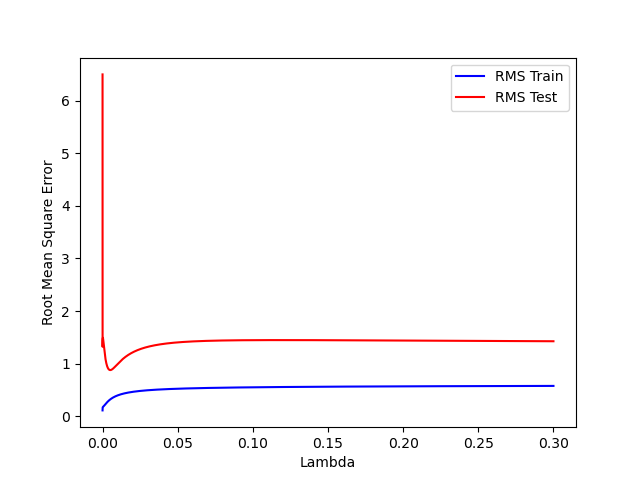
\includegraphics[scale=0.5]{img/Lambda_vs_RMS.png}
    \caption{Even with a slight increase in the regularization term $\lambda$, the RMS error on the testing set heavily decreases. }
    \label{fig:enter-label}
  \end{figure} 

\subsection{Least Squares Solution}

  Now that we have this form, we might as well just solve it. 

  \begin{theorem}[Least Squares Solution for Ridge Regression]
    The minimizer of the ridge loss is 
    \begin{equation}
      \hat{\beta} = (X^T X+ \lambda I)^{-1} X^T Y
    \end{equation}
  \end{theorem}
  \begin{proof}
    TBD
  \end{proof} 

  \begin{code}[MWS of Ridge Regression in scikit-learn]
    \noindent\begin{minipage}{.6\textwidth}
    \begin{lstlisting}[]{Code}
      import numpy as np 
      from sklearn.linear_model import Ridge  

      X = np.random.randn(10, 5) 
      y = np.random.randn(10)
      # regularization parameter
      model = Ridge(alpha=1.0)  
      model.fit(X, y) 
      print(model.score(X, y))  
      print(model.intercept_)
      print(model.coef_) 
      print(model.predict(np.array([[1, 2, 3, 4, 5]]))) 
    \end{lstlisting}
    \end{minipage}
    \hfill
    \begin{minipage}{.39\textwidth}
    \begin{lstlisting}[]{Output}
      0.8605535024325397
      -0.28291076492665157
      [-0.10400521 -0.7587073  -0.05116735  1.16236649 -0.0401323 ]
      [2.39097184]
      .
      .
      .
      .
      .
      .
    \end{lstlisting}
    \end{minipage}
  \end{code}

\subsection{Bias Variance Tradeoff}

  \begin{theorem}[Bias Variance Decomposition of Ridge Regression]
    TBD 
  \end{theorem}

  From a computational point of view, we can see that by adding the $\lambda I$ term, it \textit{dampens} the matrix so that it does become invertible (or well conditioned), allowing us to find a solution. The higher the $\lambda$ term, the higher the damping effect. 

\subsection{Concentration Bounds}

  The next theorem compares the performance of the best ridge regression estimator to the best linear predictor. 

  \begin{theorem}[Hsu, Kakade, Zhang, 2014 \cite{hsu2014random}] 
    Suppose that $||X_i|| \leq r$ and let $\beta^T x$ be the best linear approximation to $m(x)$. Then, with probability at least $1 - 4 e^{-t}$, we have
    \begin{equation}
      r(\hat{\beta}) - r(\beta) \leq \bigg( 1 + O \bigg( \frac{1 + r^2 / \lambda}{n} \bigg) \bigg) \frac{\lambda ||\beta||^2}{2} + \frac{\sigma^2}{n} \frac{\Tr(\Sigma)}{2 \lambda}
    \end{equation}
  \end{theorem}

  We can see that the $\lambda$ term exists in the numerator on $\frac{\lambda ||\beta||^2}{2}$ and in the denominator on $\frac{\Tr(\Sigma)}{2 \lambda}$. This is the bias variance tradeoff. The first term is the bias term, which is the penalty for not being able to fit the data as well. The second term is the variance term, which is the penalty for having a more complex model. So our optimal $\lambda$ in the theoretical sense would be the one that minimizes the sum of these two terms. In practice, it's not this clean since we have unknown quantities in the formula, but just like how we did cross validation over the model complexity, we can also do cross validation over the $\lambda$. The decomposition above just gives you a theoretical feeling of how these things trade off. 

\subsection{Tuning the Regularization Coefficient}
 
\section{Stepwise Regression} 

  Now we move to \textit{sparse} linear regression. 

  Now suppose that $d > n$, then the first problem is that we can no longer use least squares since $X^T X$ is no longer invertible and the same problem happens with maximum likelihood. This is known as the \textbf{high dimensional} or \textbf{large $p$, small $n$} problem. The most straightforward way is simply to reduce the covariates to a dimension smaller than $n$. This can be done with three ways. 
  \begin{enumerate}
    \item We perform PCA on the $X$ and use the first $k$ principal components where $k < n$. 
    \item We cluster the covariates based on their correlation. We can use one feature from each cluster or take the average of the covariates within each cluster. 
    \item We can screen the variables by choosing the $k$ features that have the largest correlation with $Y$. 
  \end{enumerate}
  Once this is done, we are back in the low dimensional regime and can use least squares. Essentially, this is a way to find a good subset of the covariates, which can be formalized by the following. Let $S$ be a subset of $[d]$ and let $X_S = (X_j \,:\, j \in S)$. If the size of $S$ is not too large, we can regress $Y$ on $X_S$ instead of $X$. 

\subsection{Best Subset Regression}

  \begin{definition}[Best Subset Regression]
    \textbf{Best subset regression} is a linear regression model that wants to solve the best subset $S$ that minimizes the constrained loss 
    \begin{equation}
      L(\beta, x, y) =  (y - \beta x)^2, \qquad \text{ subject to } \|\beta\|_0 \leq K
    \end{equation}
    where $\|\beta\|_0$ is the number of non-zero entries in $\beta$.\footnote{Note that $\| \cdot \|_0$ is not a norm.}
  \end{definition}

  There will be a bias variance tradeoff. As $k$ increases, the bias decreases but the variance increases. 

  The minimization of the empirical error is over all subset of size $k$, and from this fact we can expect bad news. 

  \begin{theorem}[Best Subset Regression is NP-Hard]
    Solving the best subset loss is NP-hard. 
  \end{theorem}
  \begin{proof}
    
  \end{proof}

  Even though best subset regression is infeasible, we can still approximate best subset regression in two different ways. 
  \begin{enumerate}
    \item A greedy approximation leads to \textit{forward stepwise regression}. 
    \item A convex relaxation of the problem leads to the \textit{Lasso} regression. 
  \end{enumerate}
  It turns out that the theoretical guarantees and computational time for both are the same, but the Lasso is much more popular due to having cleaner form and performing better in practice. 

\subsection{Forward Stepwise Regression} 

  Forward stepwise regression is a greedy algorithm that starts with an empty set of covariates and adds the covariate that most improves the fit. It avoids the NP-hardness of the best subset regression by adding covariates one by one. 

  \begin{definition}[Greedy Forward Stepwise Regression]
    Given your data $\mathcal{D}$, let's first standardize it to have mean $0$ and variance $1$.\footnote{This may or may not be a good idea, since the variance of each covariate can tell you a lot about the importance of the covariate.} You start off with a set $\mathcal{Q} = \{\}$ and choose the number of parameters $K$. 
    \begin{enumerate}
      \item With each covariate $X = (X_1, \ldots, X_n)$, we compute the correlation between it and the $Y$, which reduces to the inner product (since we standardized). 
      \begin{equation}
        \rho_j = \langle Y, X_{:, j} \rangle = \frac{1}{n} \sum_{i=1}^n Y_i X_{ji}
      \end{equation}

      \item Then, we take the covariate index that has the highest empirical correlation with $Y$, add it to $\mathcal{Q}$ and regress $Y$ only on this covariate. 
      \begin{equation}
        q_1 = \argmax_j \rho_j , \;\; \mathcal{Q} = \{q_1\}, \;\; \hat{\beta}_{q_1} = \argmin_{\beta} \frac{1}{n} ||Y - X_{:, q_1} \beta||^2 
      \end{equation}

      \item Then you repeat the process. You take the residual values $r = Y - X_{:, q_1} \hat{\beta}_{q_1} \in \mathbb{R}^n$ compute the correlation between $r$ and the remaining covariates, and pick our the maximum covariate index $q_2$. Then, you \textit{repeat the regression from start} with these two covariates 
      \begin{equation}
        q_2 = \argmax_j \langle r, X_{: ; j} \rangle , \;\; \mathcal{Q} = \{q_1, q_2\}, \;\; \hat{\beta}_{q_1, q_2} = \argmin_{\beta} \frac{1}{n} ||Y - X_{:,[q_1, q_2]} \beta||^2
      \end{equation}
      Note that you're not going to get the same coefficient for $\hat{\beta}_{q_1}$ as before since you're doing two variable regression. 

      \item You get out the residual values $r = Y - X_{:, [q_1, q_2]} \hat{\beta}_{q_1, q_2} \in \mathbb{R}^n$ and keep repeating this process until you have $K$ covariates in $\mathcal{Q}$. 
    \end{enumerate}
  \end{definition}

  Again, there is a bias variance tradeoff in choosing the number of covariates $K$, but through cross-validation, we can find the optimal $K$. It is also easy to add constraints, e.g. if we wanted to place a restriction that two adjacent covariates can't be chosen, we can easily add this to the algorithm. 

\subsection{Bias Variance Tradeoff}

\subsection{Concentration Bounds}

  \begin{theorem}[DeVore and Temlyakov, 1996]
    For all $f \in \mathcal{L}_1$, the residual $r_N$ after $N$ steps of OGA satisfies
    \begin{equation}
      \|r_N\| \leq \frac{\|f\|_{\mathcal{L}_1}}{\sqrt{N + 1}} \tag{4}
    \end{equation}
    for all $N \geq 1$.
  \end{theorem}
  \begin{proof}
    Note that $f_N$ is the best approximation to $f$ from $\text{Span}(V_N)$. On the other hand, the best approximation from the set $\{a g_N : a \in \mathbb{R}\}$ is $\langle f, g_N \rangle g_N$. The error of the former must be smaller than the error of the latter. In other words, $\|f - f_N\|^2 \leq \|f - f_{N-1} - \langle r_{N-1}, g_N \rangle g_N\|^2$. Thus,
    \begin{align}
      \|r_N\|^2 &\leq \|r_{N-1} - \langle r_{N-1}, g_N \rangle g_N\|^2 \\
      &= \|r_{N-1}\|^2 + |\langle r_{N-1}, g_N \rangle|^2 \|g_N\|^2 - 2|\langle r_{N-1}, g_N \rangle|^2 \\
      &= \|r_{N-1}\|^2 - |\langle r_{N-1}, g_N \rangle|^2. \tag{5}
    \end{align}

    Now, $f = f_{N-1} + r_{N-1}$ and $\langle f_{N-1}, r_{N-1} \rangle = 0$. So,
    \begin{align}
      \|r_{N-1}\|^2 &= \langle r_{N-1}, r_{N-1} \rangle = \langle r_{N-1}, f - f_{N-1} \rangle = \langle r_{N-1}, f \rangle - \langle r_{N-1}, f_{N-1} \rangle \\
      &= \langle r_{N-1}, f \rangle = \sum_j \beta_j \langle r_{N-1}, \psi_j \rangle \leq \sup_{\psi \in D} |\langle r_{N-1}, \psi \rangle| \sum_j |\beta_j| \\
      &= \sup_{\psi \in D} |\langle r_{N-1}, \psi \rangle| \|f\|_{\mathcal{L}_1} = |\langle r_{N-1}, g_N \rangle| \|f\|_{\mathcal{L}_1}.
    \end{align}

    Continuing from equation (5), we have
    \begin{align}
      \|r_N\|^2 &\leq \|r_{N-1}\|^2 - |\langle r_{N-1}, g_N \rangle|^2 = \|r_{N-1}\|^2 \left( 1 - \frac{\|r_{N-1}\|^2 |\langle r_{N-1}, g_N \rangle|^2}{\|r_{N-1}\|^4} \right) \\
      &\leq \|r_{N-1}\|^2 \left( 1 - \frac{\|r_{N-1}\|^2 |\langle r_{N-1}, g_N \rangle|^2}{|\langle r_{N-1}, g_N \rangle|^2 \|f\|_{\mathcal{L}_1}^2} \right) = \|r_{N-1}\|^2 \left( 1 - \frac{\|r_{N-1}\|^2}{\|f\|_{\mathcal{L}_1}^2} \right).
    \end{align}

    If $a_0 \geq a_1 \geq a_2 \geq \cdots$ are nonnegative numbers such that $a_0 \leq M$ and $a_N \leq a_{N-1}(1 - a_{N-1}/M)$ then it follows from induction that $a_N \leq M/(N+1)$. The result follows by setting $a_N = \|r_N\|^2$ and $M = \|f\|_{\mathcal{L}_1}^2$. $\square$
  \end{proof}

  If $f$ is not in $\mathcal{L}_1$, it is still possible to bound the error as follows.

  \begin{theorem}
    For all $f \in \mathcal{H}$ and $h \in \mathcal{L}_1$,
    \begin{equation}
      \|r_N\|^2 \leq \|f - h\|^2 + \frac{4\|h\|_{\mathcal{L}_1}^2}{N}. \tag{6}
    \end{equation}
  \end{theorem}
  \begin{proof}
    Choose any $h \in \mathcal{L}_1$ and write $h = \sum_j \beta_j \psi_j$ where $\|h\|_{\mathcal{L}_1} = \sum_j |\beta_j|$. Write $f = f_{N-1} + f - f_{N-1} = f_{N-1} + r_{N-1}$ and note that $r_{N-1}$ is orthogonal to $f_{N-1}$. Hence, $\|r_{N-1}\|^2 = \langle r_{N-1}, f \rangle$ and so
    \begin{align}
      \|r_{N-1}\|^2 &= \langle r_{N-1}, f \rangle = \langle r_{N-1}, h + f - h \rangle = \langle r_{N-1}, h \rangle + \langle r_{N-1}, f - h \rangle \\
      &\leq \langle r_{N-1}, h \rangle + \|r_{N-1}\| \|f - h\| \\
      &= \sum_j \beta_j \langle r_{N-1}, \psi_j \rangle + \|r_{N-1}\| \|f - h\| \\
      &\leq \sum_j |\beta_j| |\langle r_{N-1}, \psi_j \rangle| + \|r_{N-1}\| \|f - h\| \\
      &\leq \max_j |\langle r_{N-1}, \psi_j \rangle| \sum_j |\beta_j| + \|r_{N-1}\| \|f - h\| \\
      &= |\langle r_{N-1}, g_N \rangle| \|h\|_{\mathcal{L}_1} + \|r_{N-1}\| \|f - h\| \\
      &\leq |\langle r_{N-1}, g_N \rangle| \|h\|_{\mathcal{L}_1} + \frac{1}{2} (\|r_{N-1}\|^2 + \|f - h\|^2).
    \end{align}

    Hence,
    \begin{equation}
      |\langle r_{N-1}, g_N \rangle|^2 \geq \frac{(\|r_{N-1}\|^2 - \|f - h\|^2)^2}{4\|h\|_{\mathcal{L}_1}^2}.
    \end{equation}

    Thus,
    \begin{equation}
      a_N \leq a_{N-1} \left( 1 - \frac{a_{N-1}}{4\|h\|_{\mathcal{L}_1}^2} \right)
    \end{equation}
    where $a_N = \|r_N\|^2 - \|f - h\|^2$. By induction, the last displayed inequality implies that $a_N \leq 4\|h\|_{\mathcal{L}_1}^2/k$ and the result follows. $\square$
  \end{proof}

  \begin{corollary}
    For each $N$,
    \begin{equation}
      \|r_N\|^2 \leq \sigma_N^2 + \frac{4\theta_N^2}{N}
    \end{equation}
    where $\theta_N$ is the $\mathcal{L}_1$ norm of the best $N$-atom approximation.
  \end{corollary}

  By combining the previous results with concentration of measure arguments we get the following result, due to Barron, Cohen, Dahmen and DeVore (2008).

  \begin{theorem}
    Let $\hat{h}_n = \arg\min_{h \in \mathcal{F}_n} \|f_0 - h\|^2$. Suppose that $\limsup_{n \to \infty} \|\hat{h}_n\|_{\mathcal{L}_1,n} < \infty$. Let $N \sim \sqrt{n}$. Then, for every $\gamma > 0$, there exist $C > 0$ such that
    \begin{equation}
      \|f - \hat{f}_N\|^2 \leq 4\sigma_N^2 + \frac{C \log n}{n^{1/2}}
    \end{equation}
    except on a set of probability $n^{-\gamma}$.
  \end{theorem} 
  \begin{proof}
    
  \end{proof}

  If we square root it to compare the norm, this reduces to a rate of about $\frac{1}{\sqrt[4]{n}}$. This is the optimal rate. What this is saying that forward stepwise gets to within about $\frac{1}{\sqrt{n}}$ of what you would get if you did the perfect best subset regression. Another interesting property is that this bound is dimensionless, which makes sense since we are approximating the best $K$-term linear predictor (not the true regressor), which is a weaker claim. On the other hand, if we use nonparameteric estimators to estimate the true regressor, then we will get the curse of dimensionality. 

\subsection{Stagewise Regression} 

  Stagewise regression is a variant of forward stepwise regression where we add the covariate that most improves the fit, but we only take a small step in that direction. This is useful when we have a lot of covariates and we don't want to overfit. 

 
\section{Lasso Regression} 

  The Lasso approximates the best subset regression by using a convex relaxation. In particular, the norm $||\beta||_0$ is not convex, but the L1 norm $||\beta||_1$ is. Therefore, we want relax our constraint equation as such: 
  \begin{equation}
    \argmin_{||\beta||_0 \leq L} r(\beta) \mapsto \argmin_{||\beta||_1 \leq L} r(\beta)
  \end{equation}
  This gives us a convex problem, which we can then solve. In fact, it turns out that optimizing the risk given the L1 restriction on the norm is equivalent to minimizing the risk plus a L1 penalty, as this is the Lagrangian form of the original equation (this is in convex optimization). Therefore, there exists a pair $(L, \lambda)$ for which the two problems are equivalent 
  \begin{equation}
    \argmin_{||\beta||_1 \leq L} r(\beta) = \argmin_{\beta} r(\beta) + \lambda ||\beta||_1
  \end{equation}

  \begin{definition}[LASSO Regression]
    In \textbf{lasso regression}, we minimize the loss defined
    \begin{equation}
      \hat{R} (\beta) = \frac{1}{n} \sum_{i=1}^n (y^{(i)} - \beta^T x^{(i)})^2 + \lambda ||\beta||_1
    \end{equation}
    where we penalize according to the L1 norm of the coefficients. 
  \end{definition}

  A question arises: Why use the L1 norm? The motivation behind this is that we want to model the L0 norm as much as possible but at the same time we want it to be convex. This turns out to be precisely the L1 norm. Unfortunately, there is no closed form solution for this estimator, but in convex optimization, we can prove that this estimator is sparse. That is, for large enough $\lambda$, many of the components of $\hat{\beta}$ are $0$. The classical intuition for this is the figure below, where the equipotential lines have ``corners.'' In fact for any $0 < p < 1$, there are also corners, but the problem with using these p-norms is that they are not convex. 

  \begin{figure}[H]
    \centering 
    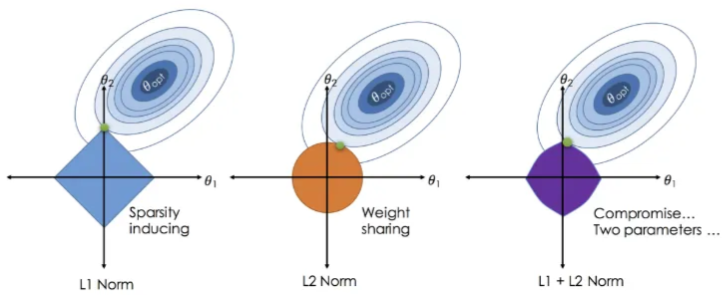
\includegraphics[scale=0.5]{img/regularizers.png}
    \caption{The ridge regularizer draws equipotential circles in our parameter space. The lasso draws a diamond, which tends to give a sparser solution since the loss is most likely to ``touch'' the corners of the contour plots of the regularizer. The elastic net is a linear combination of the ridge and lasso regularizers.} 
    \label{fig:regularizers_visual}
  \end{figure}

  To motivate this even further, let us take the two vectors 
  \begin{align}
    a = \bigg( \frac{1}{\sqrt{d}}, \ldots, \frac{1}{\sqrt{d}} \bigg) \qquad b = ( 1, 0, \ldots, 0)
  \end{align}
  Then the L0, L1, and L2 norms of $a$ are $d, \sqrt{d}, 1$ and those of $b$ are $1, 1, 1$. We want to choose a norm that capture the sparsity of $b$ and distinguishes it from $b$., The L0 norm clearly does this, but the L2 norm does not. The L1 norm is a good compromise between the two. 

  \begin{code}[MWS of Lasso Regression in scikit-learn]
    \noindent\begin{minipage}{.6\textwidth}
    \begin{lstlisting}[]{Code}
      from sklearn.linear_model import Lasso

      X = np.random.randn(10, 5) 
      y = np.random.randn(10)
      # regularization parameter
      model = Lasso(alpha=1e-1)  
      model.fit(X, y) 
      print(model.score(X, y))  
      print(model.intercept_)
      print(model.coef_) 
      print(model.predict(np.array([[1, 2, 3, 4, 5]]))) 
    \end{lstlisting}
    \end{minipage}
    \hfill
    \begin{minipage}{.39\textwidth}
    \begin{lstlisting}[]{Output}
      0.47590269719236045
      -0.8861298412689853
      [0.         0.10767647 0.24172197 0.7427863  0.        ]
      [3.02553422]
      .
      .
      .
      .
      .
    \end{lstlisting}
    \end{minipage}
  \end{code}

\subsection{Bias Variance Tradeoff}

\subsection{Concentration Bounds}

  This now raises the question of how to determine a suitable regularization parameter $\lambda$. The next theorem shows a nice concentration property of the Lasso for bounded covariates. 

  \begin{theorem}[Concentration of Lasso]
    Given $(X, Y)$, assume that $|Y| \leq B$ and $\max_j |X_j| \leq B$. Let 
    \begin{equation}
      \beta^\ast = \argmin_{||\beta||_1 \leq L} r(\beta)
    \end{equation}
    be the best sparse linear predictor in the L1 sense, where $r(\beta) = \mathbb{E}[ (Y - \beta^T X)^2]$. Let our lasso estimator be 
    \begin{equation}
      \hat{\beta} = \argmin_{||\beta||_1 \leq L} \hat{r}(\beta) = \argmin_{||\beta||_1 \leq L} \frac{1}{n} \sum_{i=1}^n (Y_i - \beta^T X_i)^2
    \end{equation}
    which minimizes the empirical risk. Then, with probability at least $1 - \delta$, 
    \begin{equation}
      r(\hat{\beta}) \leq r(\beta^\ast) + \sqrt{\frac{16(L+1)^4 B^2}{n} \log \bigg( \frac{\sqrt{2} d}{\sqrt{\delta}} \bigg)} 
    \end{equation}
  \end{theorem}
  \begin{proof}
    
  \end{proof}

\subsection{Optimization}

  Soft Thresholding and Proximal Gradient Descent
 
\section{Robust Regression}
 
\section{Bayesian Linear Regression} 

  \subsection{Regularization with Priors}

    We will now demonstrate how having a normal $\alpha \mathbf{I}$ prior around the origin in a Bayesian setting is equivalent to having a ridge penalty of $\lambda = \sigma^2 / \alpha^2$ in a frequentist setting. If we have a Gaussian prior of form 
    \[p(\mathbf{w} \mid \alpha^2) = N(\mathbf{w} \mid \mathbf{0}, \alpha^2 \mathbf{I}) = \bigg( \frac{1}{2 \pi \alpha^2} \bigg)^{M/2} \exp \bigg( -\frac{1}{2\alpha^2} ||\mathbf{w}||^2_2 \bigg)\]
    We can use Bayes rule to compute 
    \begin{align*}
        p(\mathbf{w} \mid \mathbf{X}, \mathbf{Y}, \alpha^2, \sigma^2) & \propto p(\mathbf{Y} \mid \mathbf{w}, \mathbf{X}, \alpha^2, \sigma^2) \, p(\mathbf{w} \mid \mathbf{X}, \alpha^2, \sigma^2) \\
        & = \bigg[ \prod_{n=1}^N p(y^{(n)} \mid \mathbf{w}, \mathbf{x}^{(n)}, \alpha^2, \sigma^2 )\bigg] \, p(\mathbf{w} \mid \mathbf{X}, \alpha^2, \sigma^2) \\
        & = \bigg[ \prod_{n=1}^N \frac{1}{\sqrt{2 \pi \sigma^2}} \exp \bigg( - \frac{(y^{(n)} - h_\mathbf{w} (x^{(n)}))^2}{2 \sigma^2} \bigg) \bigg] \cdot \bigg( \frac{1}{2 \pi \alpha^2} \bigg)^{M/2} \exp \bigg( -\frac{1}{2\alpha^2} ||\mathbf{w}||^2_2 \bigg)
    \end{align*}
    and taking the negative logarithm gives us 
    \[\ell(\mathbf{w}) = \frac{1}{2\sigma^2} \sum_{n=1}^N \big(y^{(n)} - h_\mathbf{w} (\mathbf{x}^{(n)}) \big)^2 + \frac{N}{2}\ln{\sigma^2} + \frac{N}{2} \ln(2\pi) - \frac{M}{2} \ln(2\pi \alpha^2) + \frac{1}{2 \alpha^2} ||\mathbf{w}||_2^2\]
    taking out the constant terms relative to $\mathbf{w}$ and multiplying by $2 \sigma^2$ (which doesn't affect optima) gives us the ridge penalized error with a penalty term of $\lambda = \sigma^2 / \alpha^2$. 
    \[E(\mathbf{w}) = \frac{1}{2} \sum_{n=1}^N \big(y^{(n)} - h_\mathbf{w} (\mathbf{x}^{(n)}) \big)^2 + \frac{\sigma^2}{\alpha^2} ||\mathbf{w}||_2^2\]
    But minimizing this still gives a point estimate of $\mathbf{w}$, which is not the full Bayesian treatment. In a Bayesian setting, we are given the training data $(\mathbf{X}, \mathbf{Y})$ along with a new test point $\mathbf{x}^\prime$ and want to evaluate the predictive distribution $p(y \mid \mathbf{x}^\prime, \mathbf{X}, \mathbf{Y})$. We can do this by integrating over $\mathbf{w}$. 
    \begin{align*}
        p(y \mid \mathbf{x}^\prime, \mathbf{X}, \mathbf{Y}) & = \int p(y \mid \mathbf{x}^\prime, \mathbf{w}, \mathbf{X}, \mathbf{Y}) \, p(\mathbf{w} \mid \mathbf{x}^\prime, \mathbf{X}, \mathbf{Y}) \, d \mathbf{w} \\
        & = \int p(y \mid \mathbf{x}^\prime, \mathbf{w}) \, p(\mathbf{w} \mid \mathbf{X}, \mathbf{Y}) \, d \mathbf{w} 
    \end{align*}
    where we have omitted the irrelevant variables, along with $\alpha^2$ and $\sigma^2$ to simplify notation. By substituting the posterior $p(\mathbf{w} \mid \mathbf{X}, \mathbf{Y})$ with a normalized version of our calculation above and by noting that 
    \[p(y \mid \mathbf{x}^\prime, \mathbf{w}) = N(y \mid h_\mathbf{w} (\mathbf{x}^\prime), \sigma^2) = \frac{1}{\sqrt{2 \pi \sigma^2}} \exp \bigg( -\frac{\big(y - h_\mathbf{w} (\mathbf{x}^\prime)\big)^2}{2 \sigma^2} \bigg)\]
    Now this integral may or may not have a closed form, but if we consider the polynomial regression with the hypothesis function of form 
    \[h_\mathbf{w} (x) = w_0 + w_1 x + w_2 x^2 + \ldots + w_{M-1} x^{M-1}\]
    then this integral turns out to have a closed form solution given by 
    \[p(y \mid \mathbf{x}^\prime, \mathbf{X}, \mathbf{Y}) = N \big( y \mid m(x^\prime), s^2 (x^\prime)\big)\]
    where 
    \begin{align*}
        m(x^\prime) & = \frac{1}{\sigma^2} \boldsymbol{\phi}(x^\prime)^T \mathbf{S} \bigg( \sum_{n=1}^N \boldsymbol{\phi}(x^{(n)}) y^{(n)} \bigg) \\
        s^2 (x^\prime) & = \sigma^2 + \boldsymbol{\phi}(x^\prime)^T \mathbf{S} \boldsymbol{\phi}(x^\prime) \\
        \mathbf{S}^{-1} & = \alpha^{-2} \mathbf{I} + \frac{1}{\sigma^2} \sum_{n=1}^N \boldsymbol{\phi}(x^{(n)}) \boldsymbol{\phi}(x^\prime)^T 
    \end{align*}
    and $\boldsymbol{\phi}(x)$ is the vector of functions $\phi_i (x) = x^i$ from $i = 0, \ldots, M-1$. 

 

\section{Generalized Linear Models} 

  Remember the linear model looked like this, where we use the conventional $\beta$ notation to represent parameters. 
  \begin{equation}
    Y = X^T \beta + \epsilon, \;\; \epsilon \sim N(0, \sigma^2 I)
  \end{equation}
  which implies that $Y \mid X \sim N(X^T \beta, \sigma^2 I)$. Basically, given $x$, I assume some distribution of $Y$, and the value of $x$ will help me guess what the mean of this distribution is. Note that we in here assume that only the mean depends on $X$. I could potentially have something crazy, like 
  \[Y \mid X \sim N(X^T \beta, (X^T \gamma) (X X^T + I))\]
  where the covariance will depend on $X$, too, but in this case we only assume that that mean is dependent on $X$. 
  \[Y \mid X \sim N(\mu(X), \sigma^2 I)\]
  where in the linear model, $\mu(X) = X^T \beta$. So, there are three assumptions we are making here: 
  \begin{enumerate}
    \item $Y \mid X$ is Gaussian. 
    \item $X$ only affects the mean of $Y \mid X$, written $\mathbb{E}[Y \mid X] = \mu(X)$. 
    \item $X$ affects the mean in a linear way, such that $\mu(X) = X^T \beta$. 
  \end{enumerate}
  So the two things we are trying to relax are: 
  \begin{enumerate}
    \item \textbf{Random Component}: the response variable $Y \mid X$ is continuous and normally distributed with mean $\mu = \mu(X) = \mathbb{E}[Y \mid X]$. 
    \item \textbf{Link}: I have a link that explains the relationship between the $X$ and the $\mu$, and this relationship is $\mu(X) = X^T \beta$. 
  \end{enumerate}
  So when talking about GLMs, we are not changing the fact that we have a linear function $X \mapsto X^T \beta$. However, we are going to assume that $Y \mid X$ now comes from a broader \textbf{family of exponential distributions}. Second, we are going to assume that there exists some \textbf{link function} $g$
  \[g(\mu(X)) = X^T \beta\]
  Admittedly, this is not the most intuitive way to think about it, since we would like to have $\mu(X) = f(X^T \beta)$, but here we just decide to call $f = g^{-1}$. Therefore, if I want to give you a GLM, I just need to give you two things: the conditional distribution $Y \mid X$, which can be any distribution in the exponential family, and the link function $g$. 

  We really only need this link function due to compatibility reasons. Say that $Y \mid X \sim \mathrm{Bern}(p)$. Then, $\mu(X) = \mathbb{E}[Y \mid X]$ always lives in $[0, 1]$, but $X^T \beta$ always lives in $\mathbb{R}$. We want our model to be realistic, and we can clearly see the problem shown in Figure \ref{fig:Bernoulli_GLM}. 

  \begin{figure}[H]
    \centering
    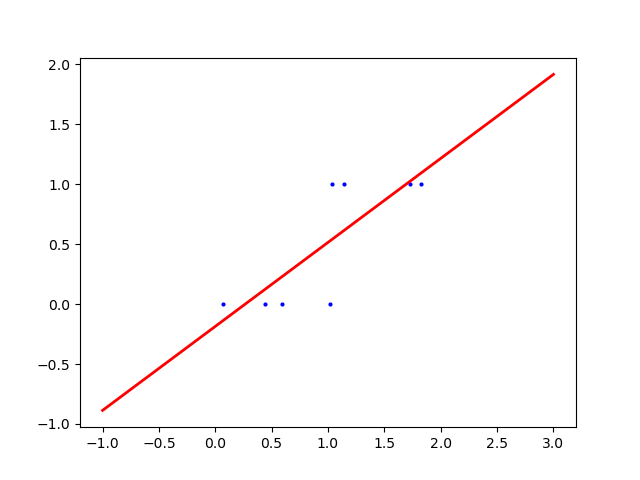
\includegraphics[scale=0.5]{img/GLM_bernoulli.png}
    \caption{Fitting a linear model for Bernoulli random variables will predict a mean that is outside of $[0, 1]$ when getting new datapoints. }
    \label{fig:Bernoulli_GLM}
  \end{figure}

  If $Y \mid X$ is some exponential distribution, then its support is always positive and so $\mu(X) > 0$. But if we stick to the old form of $\mu(X) = X^T \beta$, then $\mathrm{Im}(\mu) = \mathbb{R}$, which is not realistic when we predict negative values. Let's take a couple examples: 

  \begin{example}[Disease Epidemic]
    In the early stages of a disease epidemic, the rate at which new cases occur can often increase exponentially through time. Clearly, $\mu(X) = \mathbb{E}[Y \mid X]$ should be positive and we should have some sort of exponential trend. Hence, if $\mu(x)$ is the expected number of cases on data $x$, a model of the form 
    \begin{equation}
      \mu(x) = \gamma \exp (\delta x)
    \end{equation}
    seems appropriate, where $\gamma$ and $\delta$ are simply scaling factors. Clearly, $\mu(X)$ is not of the form $f(X^T \beta)$. So what I do is to transform $\mu$ in such a way that I can get something that is linear. 
    \begin{equation}
      \log(\mu(X)) = \log(\gamma) + \delta X
    \end{equation}
    which is now linear in $X$, of form $\beta_0 + \beta_1 X$. This will have some effects, but this is what needs to be done to have a genearlized linear model. Note that what I did to $\mu$ was take the log of it, and so the link function is $g = \log$, called the \textbf{log-link}. Now that we have chosen the $g$, we still need to choose what the conditional distribution $Y \mid X$ would be. This is determined by speaking with industry professionals, experience, and convenience. In this case, $Y$ is a count, and since this must be a discrete distribution. Since it is not bounded above, we think Poisson. 
  \end{example}

  \begin{example}[Prey Capture Rate]
    The rate of capture of preys, $Y$, by a hunting animal, tends to increase with increasing density of prey $X$, but eventually level off when the predator is catching as much as it can cope with. We want to find a perhaps concave function that levels off, and suitable model might be 
    \begin{equation}
      \mu(X) = \frac{\alpha X}{h + X}
    \end{equation}
    where $\alpha$ represents the maximum capture rate, and $h$ represents the prey density at which the capture rate is half the maximum rate. Again, we must find some transformation $g$ that turns this into a linear function of $X$, and what we can do it use the \textbf{reciprocal-link}. 
    \begin{equation}
      \frac{1}{\mu(X)} = \frac{h + X}{\alpha X} = \frac{h}{\alpha} \frac{1}{X} + \frac{1}{\alpha}
    \end{equation}
    The standard deviation of capture rate might be approximately proportional to the mean rate, suggesting the use of a Gamma distribution for the response. 
  \end{example}

  \begin{example}[Kyphosis Data]
    The Kyphosis data consist of measurements on $81$ children following corrective spinal surgery. The binary response variable, Kyphosis, indicates the presence or absence of a postoperative deforming. The three covariates are: age of the child in months, number of the vertebrae involved in the operation, and the start of the range of the vertebrae involved. The response variable is binary so there is no choice: $Y \mid X$ is Bernoulli with expected value $\mu(X) \in (0, 1)$. We cannot write $\mu(X) = X^T \beta$ because the right hand side ranges through $\mathbb{R}$, and so we find an invertible function that squishes $\mathbb{R}$ to $(0, 1)$, and so we can choose basically any CDF. 
  \end{example}

  For clarification, when writing a distribution like $\mathrm{Bernoulli}(p)$, or $\mathrm{Binomial}(n, p)$, $\mathrm{Poisson}(\lambda)$, or $N(\mu, \sigma^2)$, the hyperparameters that we usually work with we will denote as $\boldsymbol{\theta}$, and the space that this $\boldsymbol{\theta}$ lives in will denote $\Theta$. For example, for the Bernoulli, $\Theta = [0, 1]$, and for Poisson, $\Theta = [0, +\infty)$. 

  Ultimately, a GLM consists of three steps: 
  \begin{enumerate}
    \item The observed input $X$ enters the model through a linear function $\beta^T X$. 
    \item The conditional mean of response, is represented as a function of the linear combination 
      \begin{equation}
        \mathbb{E}[Y \mid X] = \mu = f(\beta^T X)
      \end{equation}
    \item The observed response is drawn from an exponential family distribution with conditional mean $\mu$. 
  \end{enumerate}

  \subsection{Exponential Family}

    We can write the pdf of a distribution as a function of the input $x$ and the hyperparameters $\theta$, so we can write $P_\theta (x) = p(\theta, x)$. For now, let's think that both $x, \theta \in \mathbb{R}$. Think of all the functions that depend on $\theta$ and $x$. There are many of them, but we want $\theta$ and $x$ to interact in a certain way. The way that I want them to interact with each other is that they are multiplied within an exponential term. Now clearly, this is not a very rich family, so we are just slapping some terms that depend only on $\theta$ and only on $x$. 
    \[p_\theta (x) = \exp(\theta x) h(x) c(\theta)\]
    But now if $\theta \in \mathbb{R}^k$ and $x \in \mathbb{R}^q$, then we cannot simply take the product nor the inner product, but what we can do is map both of them into a space that has the same dimensions, so I can take the inner product. That is, let us map $\boldsymbol{\theta} \mapsto \boldsymbol{\eta}(\boldsymbol{\theta}) \in \mathbb{R}^k$ and $\mathbf{x} \mapsto \mathbf{T}(\mathbf{x}) \in \mathbb{R}^k$, and so 
    our exponential distribution form would be generalized into something like 
    \[p_{\boldsymbol{\theta}} (\mathbf{x}) = \exp\big[ \boldsymbol{\eta}(\boldsymbol{\theta}) \cdot \mathbf{T}(\mathbf{x}) \big] h(\mathbf{x}) c(\boldsymbol{\theta})\]
    We can think of $c(\boldsymbol{\theta})$ as the normalizing term that allows us to integrate the pdf to $1$. 
    \[\int_\mathcal{X} p_{\boldsymbol{\theta}} (\mathbf{x}) = c(\boldsymbol{\theta}) \int \exp\big[\boldsymbol{\eta}(\boldsymbol{\theta}) \cdot \mathbf{T}(\mathbf{x}) \big] h(\mathbf{x})  \,d\mathbf{x}\]
    We can just push the $c(\boldsymbol{\theta})$ term into the exponential by letting $c(\boldsymbol{\theta}) = e^{-\log(c(\boldsymbol{\theta}))^{-1}}$ to get our definition. 

    \begin{definition}[Exponential Family]
      A \textbf{k-parameter exponential family} is a family of distributions with pdf/pmf of the form 
      \[p_{\boldsymbol{\theta}} (\mathbf{x}) = \exp\big[ \boldsymbol{\eta}(\boldsymbol{\theta}) \cdot \mathbf{T}(\mathbf{x}) - B(\boldsymbol{\theta}) \big] h(\mathbf{x})\]
      The $h$ term, as we will see, will not matter in our maximum likelihood estimation, so we keep it outside the exponential. 
      \begin{enumerate}
        \item $\boldsymbol{\eta}$ is called the \textbf{canonical parameter}. Given a distribution parameterized by the regular hyperparameters $\boldsymbol{\theta}$, we would like to parameterize it in a different way $\boldsymbol{\eta}$ under the function $\boldsymbol{\eta}: \Theta \rightarrow \mathbb{R}$
        \item $\mathbf{T}(\mathbf{x})$ is called the \textbf{sufficient statistic}. 
        \item $h(\mathbf{x})$ is a nonnegative scalar function. 
        \item $B(\boldsymbol{\theta})$ is the normalizing factor. 
      \end{enumerate}
    \end{definition}

    Let's look at some examples. 

    \begin{example}[Gaussian]
      If we put the coefficient into the exponential and expand the square term, we get 
      \[p_\theta (x) = \exp \bigg( \frac{\mu}{\sigma^2} \cdot x - \frac{1}{2\sigma^2} \cdot x^2 - \frac{\mu^2}{2 \sigma^2} - \log ( \sigma \sqrt{2 \pi}) \bigg)\] 
      where 
      \[\boldsymbol{\eta}(\boldsymbol{\theta}) = \begin{pmatrix} \mu /\sigma^2 \\ -1 / 2 \sigma^2 \end{pmatrix}, \; T(x) = \begin{pmatrix} x \\ x^2 \end{pmatrix}, \; B(\theta) = \frac{\mu^2}{2 \sigma^2} + \log(\sigma \sqrt{2 \pi}), \; h(x) = 1\]
      This is not a unique representation since we can take the $\log(\sqrt{2 \pi})$ out of the exponential, but why bother to do this when we can just stuff everything into $B$ and keep $h$ simple. 
    \end{example}

    \begin{example}[Gaussian with Known Variance]
      If we have known variance, we can write the Gaussian pdf as 
      \[p_\theta (x) = \exp \bigg[ \frac{\mu}{\sigma} \cdot \frac{x}{\sigma} - \frac{\mu^2}{2 \sigma^2} \bigg] \cdot \frac{1}{\sigma \sqrt{2\pi}} e^{x^2/2 \sigma^2}\]
      where 
      \[\eta(\theta) = \frac{\mu}{\sigma}, \; T(x) = \frac{x}{\sigma}, \; B(\theta) = \frac{\mu^2}{2 \sigma^2}, \; h(x) = \frac{1}{\sigma \sqrt{2 \pi}} e^{x^2/2 \sigma^2}\]
    \end{example}

    \begin{example}[Bernoulli]
    The pmf of a Bernoulli with $\theta$ is 
    \begin{align*}
        p_\theta (x) & = \theta^x (1 - \theta)^{(1 - x)} \\
        & = \exp \big[x \log (\theta) + (1 - x)\log(1 - \theta) \big] \\
        & = \exp \bigg( x \log \Big[ \frac{\theta}{1 - \theta} \Big] - \log \Big[ \frac{1}{1 - \theta} \Big] \bigg)
    \end{align*}
    where 
    \[\eta(\theta) = \log \Big[ \frac{\theta}{1 - \theta} \Big], \; T(x) = x, \; B(\theta) = \log \Big[ \frac{1}{1 - \theta} \Big], \; h(x) = 1\]
    \end{example}


    \begin{example}[Binomial with Known Number of Trials]
    We can transform a binomial with known $N$ as 
    \begin{align*}
      p_\theta (x) &  = \binom{N}{x} \theta^x  (1 - \theta)^{1 - x} \\
                   & = \exp \bigg[ x \ln \big( \frac{\theta}{1 - \theta} \Big) + \ln(1 - \theta) \bigg] \cdot \binom{N}{x} 
    \end{align*}
    where 
      \[\eta (\theta) = \ln \big( \frac{\theta}{1 - \theta} \Big), \; T(x) = x, \; B(\theta) = \ln(1 - \theta), \; h(x) = \binom{N}{x}\]
    \end{example}

    \begin{example}[Poisson]
    The pmf of Poisson with $\theta$ can be expanded 
    \begin{align*}
        p_\theta & = \frac{\theta^{-x}}{x!} e^{-\theta} \\
        & = \exp \big[ -\theta + x\log(\theta) - \log(x!) \big] \\
        & = \exp \big[ x \log(\theta) - \theta \big] \, \frac{1}{x!}
    \end{align*}
    where 
    \[\eta(\theta) = \log(\theta), \; T(x) = x, \; B(\theta) = \theta, \; h(x) = \frac{1}{x!}\]
    \end{example}

    However, the uniform is not in here. In fact, any distribution that has a support that does not depend on the parameter is not an exponential distribution. 

    Let us now focus on one parameter families where $\theta \in \Theta \subset \mathbb{R}$, which do not include the Gaussian (with unknown mean and variance, Gamma, multinomial, etc.), which has a pdf written in the form 
    \[p_\theta (x) = \exp \big[ \eta (\theta) \, T(x) - B(\theta) \big] \, h(x)\]


    \subsubsection{Canonical Exponential Family}

      Now a common strategy in statistical analysis is to reparamaterize a probability distribution. Suppose a family of probability distributions $\{P_\theta\}$ is parameterized by $\theta \in \Theta \subset \mathbb{R}$. If we have an invertible function $\eta: \Theta \rightarrow \mathcal{T} \subset \mathbb{R}$, then we can paramaterize the same family with $\eta$ rather than $\theta$, with no loss of information. Typically, it is the case that $\eta$ is invertible for exponential families, so we can just reparameterize the whole pdf and write 
      \[p_\eta (x) = \exp \big[ \eta \, T(x) - \phi(\eta) \big] \, h(x)\]
      where $\phi = B \circ \eta^{-1}$. 

      \begin{definition}[Canonical One-Parameter Exponential Family]
      A family of distributions is said to be in \textbf{canonical one-parameter exponential family} if its density is of form 
      \[p_\eta (x) = \exp \big[ \eta \, T(x) - \phi(\eta) \big] \, h(x)\]
      which is a subfamily of the exponential family. The function $\psi$ is called the \textbf{cumulant generating function}. 
      \end{definition}

      Before we move on, let us just provide a few examples. 

      \begin{example}[Poisson]
      The Poisson can be represented as 
      \[p_\theta (x) = \exp \big[ x \log{\theta} - \theta \big] \, \frac{1}{x!}\]
      Now let $\eta = \log{\theta} \implies \theta = e^{\eta}$. So, we can reparamaterize the density as 
      \[p_\eta(x) = \exp \big[ x \eta - e^\eta \big] \, \frac{1}{x!}\]
      where $P_\eta = \mathrm{Poisson}(e^\eta)$ for $\eta \in \mathcal{T} = \mathbb{R}$, compared to $P_\theta = \mathrm{Poisson}(\theta)$ for $\theta \in \Theta = \mathbb{R}^+$. 
      \end{example}

      \begin{example}[Gaussian]
      Recall that the Gaussian with known parameter $\sigma^2$ and unknown $\theta = \mu$ is in the exponential family, since we can expand it as 
      \[p_\theta (x) = \exp \bigg[ \frac{\mu}{\sigma^2} \cdot x - \frac{\mu^2}{2 \sigma^2} \bigg] \cdot \frac{1}{\sigma \sqrt{2\pi}} e^{x^2/2 \sigma^2}\]
      We can perform the change of parameter $\eta = \mu^2 / 2\sigma^2 \implies \mu = \sigma^2 \eta$, and substituting this in will give the canonical representation 
      \[p_\eta (x) = \exp \Big[ \eta x - \frac{\sigma^2 \eta^2}{2} \Big] \cdot \frac{1}{\sigma \sqrt{2\pi}} e^{x^2/2 \sigma^2}\]
      where now $P_\eta = N(\sigma^2 \eta, \sigma^2)$ for $\eta \in \mathcal{T} = \mathbb{R}$, compared to $P_\theta = N(\theta, \sigma^2)$ for $\theta \in \Theta = \mathbb{R}$, which is basically the same space. 
      \end{example}

      \begin{example}[Bernoulli]
      The Bernoulli has an exponential form of 
      \[p_\theta (x) = \exp \bigg[ x \log \Big( \frac{\theta}{1 - \theta} \Big) + \log(1 - \theta)\bigg]\]
      Now setting $\eta = \log\big( \frac{\theta}{1 - \theta} \big) \implies \theta = \frac{1}{1 + e^{-\eta}}$, and so $B(\theta) = - \log(1 - \theta) = - \log \big( \frac{e^{-\eta}}{1 + e^{-\eta}} \big) = \log(1 + e^\eta) = \psi(\eta)$, and so the canonical paramaterization is 
      \[p_\eta (x) = \exp \big[ x \eta - \log(1 + e^{\eta}) \big]\]
      \end{example}


      We present two useful properties of the exponential family. 

      \begin{theorem}[Moments]
      Let random variable $X$ be in the canonical exponential family $P_\eta$ 
      \[p_\eta (x) = e^{\eta T(x) - \psi(\eta)} h(x)\]
      Then, the expectation and variance are encoded in the cumulant generating function in the following way 
      \[\mathbb{E} [T(X)] = \psi^\prime (\eta) \;\;\;\;\;\;\;\; \Var[T(X)] = \psi^{\prime\prime} (\eta)\]
      \end{theorem}
      \begin{proof}

      \end{proof}

      \begin{example}
      We show that this is consistent with the Poisson, normal, and Bernoulli distributions. 
      \begin{enumerate}
          \item In the Poisson, $\psi(\eta) = e^{\eta}$, and so $\psi^\prime(\eta) = e^\eta = \theta = \mathbb{E}[X]$. Taking the second derivative gives $\psi^{\prime\prime}(\eta) = e^\eta = \theta = \Var[X]$, too. \
          
          \item In the Normal with known variance $\sigma^2$, we have $\psi(\eta) = \frac{1}{2} \sigma^2 \eta^2$. So 
          \begin{align*}
              \mathbb{E}[X] & = \psi^\prime (\eta) = \sigma^2 \eta = \mu \\
              \Var[X] & = \psi^{\prime\prime} (\eta) = \sigma^2
          \end{align*}

          \item In the Bernoulli, we have $\psi(\eta) = \log(1 + e^{-\eta})$. Therefore, 
          \begin{align*}
              \mathbb{E}[X] & = \psi^\prime (\eta) = \frac{x^\eta}{1 + x^{\eta}} = \frac{1}{1 + e^{-\eta}} = \theta \\
              \Var[X] & = \psi^{\prime\prime} (\eta) = -\bigg(\frac{1}{1 + e^{-\eta}}\bigg)^2 \, e^{-\eta} \cdot -1 = \theta^2 \cdot \frac{1 - \theta}{\theta} = \theta (1 - \theta) 
          \end{align*}
      \end{enumerate}
      \end{example}

      \begin{theorem}[Convexity]
      Consider a canonical exponential family with density 
      \[p_\eta (x) = e^{\eta T(x) - \psi(\eta)} h(x)\]
      and natural parameter space $\mathcal{T}$. Then, the set $\mathcal{T}$ is convex, and the cumulant generating function $\psi$ is convex on $\mathcal{T}$. 
      \end{theorem}
      \begin{proof}
      This can be proven using Holder's inequality. However, from the theorem above, note that $\Var[T(X)] = \psi^{\prime\prime}(\eta)$ must be positive since we are talking about variance. This implies that the second derivative of $\psi$ is positive, and therefore must be convex. 
      \end{proof}

      We will look at a subfamily of the exponential family. Now remember that we introduce the functions $\boldsymbol{\eta}$ and $\mathbf{T}$ so that we can capture a much broader range of distributions, but if we have one parameter $k = 1$, then we can just set $\boldsymbol{\eta}(\boldsymbol{\theta})$ to be the new parameter $\theta$. The \textbf{canonical exponential family} for $k = 1, y \in \mathbb{R}$, is defined to have the pdf 
      \begin{equation}
        f_\theta (y) = \exp \bigg( \frac{y \theta - b(\theta)}{\phi} + c(y, \phi) \bigg)
      \end{equation}
      where 
      \begin{equation}
        h(y) = \exp \big( c(y, \phi)\big)
      \end{equation}
      If $\phi$ is known, this is a one-parameter exponential family with $\theta$ being the \textbf{canonical parameter}, and if $\phi$ is unknown, the $h(y)$ term will not depend on $\theta$, which we may not be able to split up into the exponential pdf form. In this case $\phi$ is called the \textbf{dispersion parameter}. For now, we will always assume that $\phi$ is known. 

      We can prove this for all other classes, too. We can think of the $c(y, \phi)$ as just a term that we stuff every other term into. What really differentiates the different distributions of the canonical exponential family is the $b(\theta)$. The form of $b$ will determine whether this distribution is a Gaussian, or a Bernoulli, or etc. This $b$ will capture information about the mean, the variance, the likelihood, about everything. 

      \subsection{Cumulant Generating Function}

        \begin{definition}[Score]
        The \textbf{score} is the gradient of the log-likelihood function with respect to the parameter vector. That is, given that $L(\boldsymbol{\theta})$ is the likelihood, then 
        \[s(\boldsymbol{\theta}) \coloneqq \frac{\partial \log L(\boldsymbol{\theta}; \mathbf{x})}{\partial \boldsymbol{\theta}}\]
        which gives a row covector. 
        \end{definition}

        Now, remember that the score also depends on the observations $\mathbf{x}$. If we rewrite the likelihood as a probability density function $L(\boldsymbol{\theta}; \mathbf{x}) = f(\mathbf{x}; \boldsymbol{\theta})$, then we can say that the expected value of the score is equal to $0$, since 
        \begin{align*}
         \mathbb{E}[s(\boldsymbol{\theta})] & = \int_\mathcal{X} f(\mathbf{x}; \boldsymbol{\theta}) \frac{\partial}{\partial \boldsymbol{\theta}} \log L (\boldsymbol{\theta}; \mathbf{x}) \,d\mathbf{x} \\
         & = \int_\mathcal{X} f(\mathbf{x}; \boldsymbol{\theta}) \frac{1}{f(\mathbf{x}; \boldsymbol{\theta})} \, \frac{\partial f(\mathbf{x}; \boldsymbol{\theta})}{\partial \boldsymbol{\theta}} \,dx \\
         & = \frac{\partial}{\partial \boldsymbol{\theta}} \int_\mathcal{X} f(\mathbf{x}; \boldsymbol{\theta}) \,d \mathbf{x} \\
         & = \frac{\partial}{\partial \boldsymbol{\theta}} 1 = 0
        \end{align*}
        where we take a leap of faith in switching the derivative and integral in the penultimate line. Furthermore, we can get the second identity 
        \[\mathbb{E}\bigg[ \frac{\partial^2 \ell}{\partial \theta^2} \bigg] + \mathbb{E} \bigg[ \frac{\partial \ell}{\partial \theta} \bigg]^2 = 0\]

        We can apply these two identities as follows. Since 
        \[\ell (\theta) = \frac{Y \theta - b(\theta)}{\phi} + c(Y ; \phi)\]
        therefore 
        \[\frac{\partial \ell}{\partial \theta} = \frac{Y - b^\prime(\theta)}{\phi}\]
        which yields 
        \[0 = \mathbb{E} \bigg[ \frac{\partial \ell}{\partial \theta} \bigg] = \frac{\mathbb{E}[Y] - b^\prime(\theta)}{\phi} \implies \mathbb{E}[Y] = \mu = b^\prime(\theta)\]
        On the other hand, we have 
        \[\frac{\partial^2 \ell}{\partial \theta^2} + \bigg( \frac{\partial \ell}{\partial \theta} \bigg)^2 = -\frac{b^{\prime\prime} (\theta)}{\phi} + \bigg(\frac{Y - b^\prime (\theta)}{\phi} \bigg)^2\]
        and from the previous result, we get 
        \[\frac{Y - b^\prime(\theta)}{\phi} = \frac{Y - \mathbb{E}[Y]}{\phi}\]
        together with the second identity, yields 
        \[0 = -\frac{b^{\prime\prime}(\theta)}{\phi} + \frac{\Var(Y)}{\phi^2} \implies \Var(Y) = \phi \, ^{\prime\prime} (\theta)\]
        Since variance is always positive, this implies that $b^{\prime\prime} > 0$ and therefore $b$ must be convex. 

  \subsection{Link Functions}

    Now let's go back to GLMs. In linear models, we said that the conditional expectation of $Y$ given $X = \mathbf{x}$ must be a linear function in $x$ 
    \[\mathbb{E}[Y \mid X = \mathbf{x}] = \mu(\mathbf{x}) = \mathbf{x}^T \beta\]
    But if the conditional distribution takes values in some subset of $\mathbb{R}$, such as $(0, 1)$, then it may not make sense to write this as a linear function, since $X^T \beta$ has an image spanning $\mathbb{R}$. So what we need is a link function that relates, i.e. transforms the restricted subset of $\mu$, onto the real line, so that now you can express it of the form $X^T \beta$. 
    \[g \big( \mu(X) \big) = X^T \beta\]
    Again, it is a bit more intuitive to talk about $g^{-1}$, which takes our $X^T \beta$ and transforms it to the values that I want, so we will talk about both of them simultaneously. If $g$ is our link function, we want it to satisfy 3 requirements: 
    \begin{enumerate}
        \item $g$ is continuously differentiable 
        \item $g$ is strictly increasing 
        \item $\mathrm{Im}(g) = \mathbb{R}$, i.e. it spans the entire real line
    \end{enumerate}
    This implies that $g^{-1}$ exists, which is also continuously differentable and is strictly increasing. 

    \begin{example}
    If I have a conditional distribution... 
    \begin{enumerate}
        \item that is Poisson, then we want our $\mu$ to be positive, and so we need a link function $g: \mathbb{R}^+ \rightarrow \mathbb{R}$. One choice would be the logarithm 
        \[g(\mu(X)) = \log \big( \mu(X) \big) = X^T \beta\]

        \item that is Bernoulli, then we want our $\mu$ to be in $(0, 1)$ and we need a link function $g: (0, 1) \rightarrow \mathbb{R}$. There are 2 natural choices, which may be the \textbf{logit} function 
        \[g(\mu(X)) = \log \bigg( \frac{\mu(X)}{1 - \mu(X)} \bigg) = X^T \beta\]
        or the \textbf{probit} function 
        \[g(\mu(X)) = \Phi^{-1} \big(\mu(X)\big) = X^T \beta \]
        where $\Phi$ is the CDF of a standard Gaussian. The two functions can be seen in Figure \ref{fig:logit_probit}. 
        \begin{figure}[H]
            \centering
            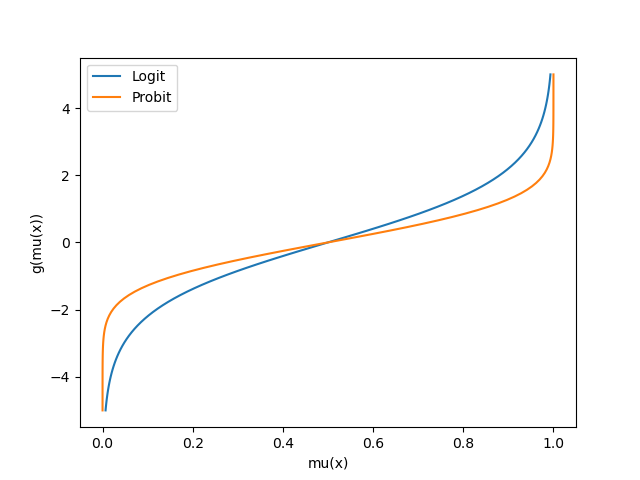
\includegraphics[scale=0.5]{img/probit_logit.png}
            \caption{Logit and Probit Functions}
            \label{fig:logit_probit}
        \end{figure}
    \end{enumerate}
    \end{example}

    Now there are many choices of functions we can take. In fact, if $\mu$ lives in $(0, 1)$, then we can really just take our favorite distribution that has a density that is supported everywhere in $\mathbb{R}$ and take the inverse cdf as our link. So far, we have no reason to prefer one function to another, but in the next section, we will see that there are more natural choices. 

    \subsubsection{Canonical Link Functions}

      Now let's summarize what we have. We assume that the conditional distribution $Y \mid X = x$ follows a distribution in the exponential family, which we can completely characterize by the cumulant generating function $\psi$. For different values of $x$, the conditional distribution will be paramaterized by different $\eta (x)$, and the resulting distribution $P_\eta$ will have some mean $\mu(x)$, which is usually not the natural parameter $\eta$. Now, let's forget about our knowledge that $\psi^\prime(\eta) = \mu$, but we know that there is some relationship between $\eta \leftrightarrow \mu$.

      Given an $x$, I need to use the linear predictor $x^T \beta$ to predict $\mu(x)$, which can be done through the link function $g$. 
      \[g\big( \mu(x) \big) = x^T \beta\]
      Now what would be a natural way of choosing this $g$? Note that our natural parameter $\eta$ for this canonical family takes value on the entire real line. I must construct a function $g$ that maps $\mu$ onto the entire real line, and so why not make it map to $\eta$. Therefore, we have 
      \[\eta(x) = g\big( \mu(x) \big) = x^T \beta\]

      \begin{definition}[Canonical Link]
      The function $g$ that links the mean $\mu$ to the canonical parameter $\theta$ is called the \textbf{canonical link}. 
      \[g(\mu) = \theta\]
      Now using our knowledge that $\psi^\prime(\eta) = \mu$, we can see that 
      \[g = (\psi^\prime)^{-1}\]
      This is indeed a valid link function. 
      \begin{enumerate}
          \item $\psi^{\prime\prime} > 0$ since it models the variance, and so $\psi^\prime$ is strictly increasing and so $g = (\psi^\prime)^{-1}$ is also strictly increasing. 
          \item The domain of $\psi^\prime$ is the real line since it takes in the natural parameter $\eta$ which exists over $\mathbb{R}$, so $\mathrm{Im}(g) = \mathbb{R}$. 
      \end{enumerate}
      \end{definition}

      So, given our cumulant generating function $\psi$ and our link function $g$, both satisfying 
      \[\psi^\prime (\eta) = \mu \text{ and } g(\mu) = x^T \beta\]
      we can combine them to get 
      \[(g \circ \psi^\prime) (\eta) = g(\mu) = x^T \beta\]
      and so, even though the mean of the response variable is not linear with respect to $x$, the value of $(g \circ \psi^\prime) (\eta)$ is indeed linear. In fact, if we choose the canonical link, then the equation 
      \[\eta = x^T \beta\]
      means that the natural parameter of our conditional distribution in the exponential family is linear with respect to $x$! From this we can find the conditional mean $\mu(x)$. 

      The reason we focus on canonical link functions is because, when the canonical link is used, the components of the model (the parameters of the linear predictor) have an additive effect on the response variable in the transformed (linked) scale, which makes the interpretation of the results easier. It's also worth noting that while using the canonical link function has some desirable properties, it is not always the best or only choice, and other link functions may be used if they provide a better fit for the data or make more sense in the context of the problem at hand.

      Let us evaluate some canonical link functions. 

      \begin{example}
      The Bernoulli has the canonical exponential form of 
      \[p_\eta (x) = \exp \big[ x \eta - \log (1 + e^\eta) \big]\]
      where $\eta = \log \big( \frac{\theta}{1 - \theta} \big)$. Since we have prior knowledge that $\theta = \mu$ (i.e. the expectation of a Bernoulli is the hyperparameter $\theta$ itself), we have a function that maps $\mu \mapsto \eta$. 
      \[\eta = g(\mu) = \log \bigg( \frac{\mu}{1 - \mu} \bigg)\]
      which gives us our result. We can also take the inverse of $\psi^\prime = \frac{e^\eta}{1 + e^\eta}$ to get our result 
      \[g (\mu) = (\psi^\prime)^{-1} (\mu) = \log \bigg( \frac{\mu}{1 - \mu} \bigg) \]
      \end{example}

  \subsection{Likelihood Optimization}

    Now let us have a bunch of data points $\{(x_n, y_n)\}_{n=1}^N$. By our model assumption, we know that the conditional distribution $Y \mid X = x_n$ is now of an exponential family with parameter $\eta_n = \eta (x_n)$ and density 
    \[p_{\eta_n} (y_n) = \exp \big[ y_n \eta_n - \psi(\eta_n) \big] h(y_n)\]
    Now we want to do likelihood optimization on $\beta$ (not $\eta$ or $\mu$), and to do this, we must rewrite the density function in a way so that it depends on $\beta$. Given a link function $g$, note the following relationship between $\beta$ and $\eta$: 
    \begin{align*}
        \eta_n = \eta (x_n) & = (\psi^\prime)^{-1} (\mu (x_n)) \\
        & = (\psi^{\prime})^{-1} \big( g^{-1} (x_n^T \beta )\big) \\
        & = h(x_n^T \beta) 
    \end{align*}
    where for shorthand notation, we define $h \coloneqq (g \circ \psi^\prime)^{-1}$. Subtituting this into the above likelihood, taking the product of all $N$ samples, and logarithming the equation gives us the following log likelihood to optimize over $\beta$. 
    \[\ell(\beta) = \log \prod_{n=1}^N p_{\eta_n} (y_n) = \sum_{n=1}^N y_n h(x_n^T \beta)  - \psi(h(x_n^T \beta) )\]
    where we dropped the $h(y_n)$ term at the end since it is a constant and does not matter. If $g$ was the canonical link, then $h$ is the identity, and we should have a linear relationship between $\eta (x_n) = x_n^T \beta$. This means that the $\eta_n$ reduces only to $x_n^T \beta$, which is much more simple to optimize. 
    \[\ell(\beta) = \log \prod_{n=1}^N p_{\eta_n} (y_n) = \sum_{n=1}^N y_n x_n^T \beta - \psi(x_n^T \beta)\]
    Note that the first term is linear w.r.t $\beta$, and $\psi$ is convex, so the entire sum must be concave w.r.t. $\beta$. With this, we can bring in some tools of convex optimization to solve. 



\bibliography{./bibfile}
\bibliographystyle{alpha}
\end{document}
